% ====================================================
%   Copyright (C)2019 All rights reserved.
%
%   Author        : Xin-Xin Ma
%   Email         : xxmawhu@163.com
%   File Name     : ds_to_ppbarenu.tex
%   Last Modified : 2019-12-25 20:33
%   Describe      :
%
% ====================================================%
\chapter{寻找奇异粲介子的稀有衰变过程$D_{s}^{+} \to p \bar{p} e^{+} \nu_{e}$}%
\label{cha:ds_ppbarenu}
本章讨论的是在BESIII寻找$D_{s}^{+}$的稀有衰变$D_{s}^{+} \to p \bar{p}
e^{+} \nu_{e}$。
受相空间的限制,$D^{+}$和$D^{0}$均不能衰变到重子对。只有Ds可能
通过三种衰变方式产生重子对,它们分别是
\begin{align}
    D_{s}^{+} &\to p \bar{n} \\
    D_{s}^{+} &\to p \bar{p} e^{+} \nu_{e} \\
    D_{s}^{+} &\to n \bar{n} e^{+} \nu_{e}
\end{align}
前者被CLEOc首先发现~\cite{Athar:2008ug},分支比的实验结果为$(1.30 \pm
0.4)\times 10^{-3}$, 随后被BESIII加以确实\cite{Ablikim:2018iad},
分支比的测量精度得到了提高,实验结果为
$\mathcal{B}(D_{s}^{+} \to p \bar{p} e^{+} \nu_e) = (1.21 \pm 0.10 \pm
0.05)\times 10^{-3}$,远远超过了理论家的预期。
后两者仍未被发现,但是中子由于在探测器中难以留下径迹,探测效率极低,
因此本文致力
于寻找 $ D_{s}^{+} \to p \bar{p} e^{+}
\nu_{e}$。该过程的机制主要来自介子交换相互作用,交换的介子包括$\eta$, $\eta
\prime$, $f(980)$,
$X(1835)$\cite{Cheng:2017qpv}。示意图为\ref{fig:meson-exchange},
理解$X(1835)$的本质对分支比的计算至关重要,这也是我们的动机之一。

\begin{figure}[htpb]
    \centering
    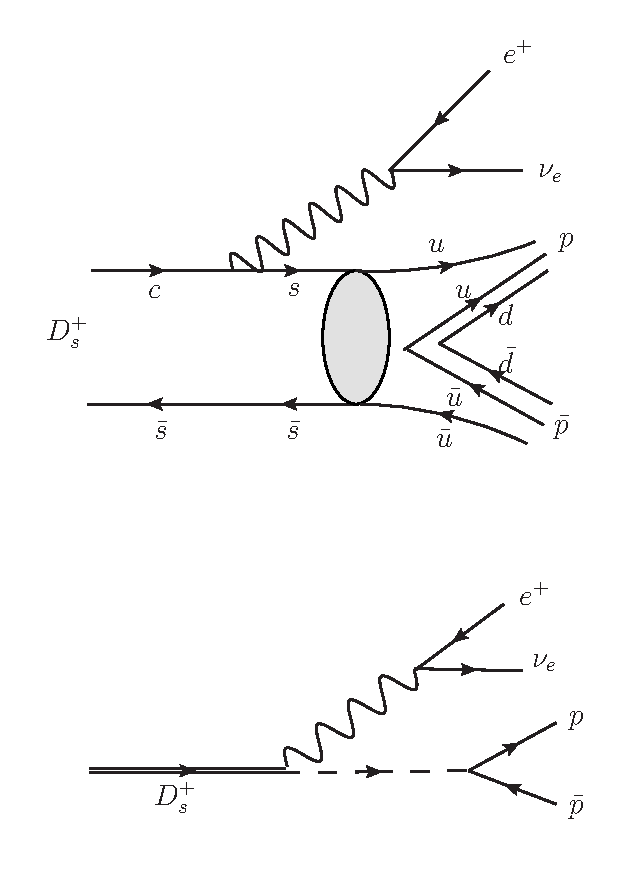
\includegraphics[width=0.8\linewidth]{dsToPPbar/intr/meson-exchange.eps}
    \caption{由介子交换引起的衰变$D_{s}^{+} \to p \bar{p} e^{+} \nu_{e}$
    示意图。}%
    \label{fig:meson-exchange}
\end{figure}
本文将从数据样本、测量方法、
信号重建、测量结果、系统误差分析出发介绍对
$D_{s}^{+} \to p \bar{p} e^{+} \nu_{e}$的寻找。

\section{测量方法}\label{sec:method}
由于相空间的限制,末态粒子的能量都较低,其中电子的能量最低,大约90MeV/c,很难被
探测器重建出来。另外中微子不能被探测器重建。面对重重困难,我们另辟蹊径,
决定在双标记方法的基础上采取
部分重建算法。首先我们选择若干个分支比大、本底低的衰变道重建一个$D_{s}^{-}$
介子,这样的衰变道称之为单标记道,被重建出的介子称为单标记$D_{s}^{-}$。单标记
道的选取原则和具体的挑选过程将在后文中详细介绍。接着我们在剩余的径迹里挑选选
出所关心的信号。由于质子和其他带电粒子的之间的误鉴别率很低,一对相交的电荷相反
的径迹被鉴别为质子对可以作为信号存在的强有力证据,我们仍旧把单标记$D_{s}^{-}$
的不变质量作为观测里来获取信号的产额。

\subsection{分支比的计算公式}

\section{样本}\label{sec:sample}
\subsection{数据样本}
数据样本选用2016年在能量点4.178GeV采集的数据,积分亮度为3.19fb,其中的opencharm末态
$D^{+}D_{s}^{*-}$是用了寻找$D_{s}^{+}$介子的衰变过程。

\subsection{模拟样本}
\subsubsection*{Generic MC}
BESIII产生的蒙特卡洛样本重要用来做本底估计,主要的成份在表~\ref{tab:generic
mc}列出
\begin{table}[htpb]
    \centering
    \caption{Generic 蒙特卡洛样本的主要构成}%
    \label{tab:generic-mc}
    \begin{tabular}{l  c  c  c}
        \toprule 
        物理过程 & 截面  &产生子 & 模拟亮度/数据亮度 \\
        \midrule 
        $D^{0} \bar{D}^{0}$             & 0.179 & BesEvtGen + conExc & 40 x \\
        $D^{+} D^{-}$                   & 0.197 & BesEvtGen + conExc & 40 x \\
        $D^{0} \bar{D}^{*0} + c.c$      & 1.211 & BesEvtGen + conExc & 40 x \\
        $D^{+} \bar{D}^{*-} + c.c$      & 1.296 & BesEvtGen + conExc & 40 x \\
        $D^{*0} \bar{D}^{*0} $          & 2.173 & BesEvtGen + conExc & 40 x \\
        $D_{s}^{+} D_{s}^{-} $          & 0.007 & BesEvtGen + conExc & 40 x \\
        $D \bar{D}^{*}\pi^{\pm} + c.c $ & 0.383 & BesEvtGen + conExc & 40 x \\
        $D \bar{D}^{*}\pi^{0} + c.c $   & 0.192 & BesEvtGen + conExc & 40 x \\
        $D \bar{D}\pi^{\pm} + c.c $     & 0.050 & BesEvtGen + conExc & 40 x \\
        $D \bar{D}\pi^{0} + c.c $       & 0.025 & BesEvtGen + conExc & 40 x \\
        \midrule 
        $e^{+} e^{-} \to q\bar{q}(u, d, s)$ & 13.8 & KKMC & 40 x \\
        \midrule 
        $e^{+}e^{-} \to \gamma_{ISR} J/\psi$     & 0.40 & KKMC & 40 x \\
        $e^{+}e^{-} \to \gamma_{ISR} \psi(3686)$ & 0.42 & KKMC & 40 x \\
        $e^{+}e^{-} \to \gamma_{ISR} \psi(3770)$ & 0.06 & KKMC & 40 x \\
        \midrule 
        $e^{+}e^{-} \to e^{+} e^{-} $       & 423.99 & Babayaga & 0.4 x \\
        $e^{+}e^{-} \to \mu^{+} \mu^{-} $   & 5.24   & Babayaga & 40 x \\
        $e^{+}e^{-} \to \tau^{+} \tau^{-} $ & 3.45   & KKMC & 40 x \\
        \midrule
        two-photon fusion & 1.7 & BesTwogam & 40 x \\
        $\pi \pi (\psi(2S)/h_{c}/J/\psi), (KK/\eta)J/\psi$ & 0.1 & BesEvtGen +
        conExc & 40 x \\
        \bottomrule
    \end{tabular}
\end{table}
\subsubsection{信号模型}
$p\bar{p}$可能不是由直接衰变而来,而是通过一个共振态间接产生。其一,此时的
$p\bar{p}$刚好能构成$X(1835)$,这时共振态的贡献将远大于非共振态,
很多分波分析都验证了这个结论。其二,
多数的半轻过程显示了非共振态的成分要比共振态低的多。因此,我们假定
$D_{s}^{+} \to X e^{+} \nu_{e}$, $X\to p \bar{p}$,其中$X$为中间共振态,可能是赝标量、矢量粒子或者更高自旋的粒子。

\begin{figure}[htbp]
      \centering
          \begin{overpic}[width=8cm]{dsToPPbar/producFeymann.eps}
              \put(10,20){\small {$D_{s}^{+}$}}
              \put(45,20){\small {$X(p\bar{p})$}}
              %\put(45,20){\small {$\eta _{1760}$}}
              %\put(45,15){\small {$f_{2,1810}$}}
              \put(30,8){$\bar{s}$}
              \put(15,32){$c$}
              \put(47,32){$s$}
              \put(87,43){$\nu_e$}
              \put(87,54){$e^{+}$}
              \put(103,30) {$p$}
              \put(103,4) {$\bar{p}$}
          \end{overpic}    
      \caption{$p\bar{p}$对产生示意图。$D_{s}^{+}$介子释放一个$W$玻色子并产生
      共振态$X(p\bar{p})$,这个共振态瞬间产生$p\bar{p}$对。
      }%
      \label{fig:feynman-diagram}
  \end{figure}
这个过程的转移动量依赖的分宽度形式为
\begin{equation}
    \frac{d \Gamma(D^{+}_{s} \to X e^{+} \nu_{e})}{d q^{2}}
    = \frac{G_{F}^{2} |V_{cs}|^{2}}{24 \pi^{3}} p_{X}^{3} |f_{+}(q^{2})|^{2}
\end{equation}
其中$G_{F}$为费米常数,$|V_{cs}|$为CKM矩阵元,$p_{X}$为共振态在$D_{s}^{+}$质心系下的动量大小,$q$是转移动量为$D_{s}^{+}$
和$X$的动量的差, $f_{+}(q^{2})$是形状因子。我们采用ISGW2模型来描述$f_{+}(q^{2})$,其形式为
\begin{equation}
    \label{eq:f_q2}
    f_{+}(q^2) = f_+(q^{2}_{\rm \max}) \left( 1 + r^{2} /12 (q^{2}_{\rm max} - q^{2}) \right)^{-1},
\end{equation}
其$r$是的有效半径,$q_{\rm \max}^{2}$是$q^{2}$的在$D_{s}^{+}$衰变运动学
约束下最大值。
我们用这个模型来产生信号蒙特卡洛样本模拟样本以进行进一步的研究工作。
为了讨论模型不确定带来的影响,我们分别采用了不同宽度、不同质量、不同自旋的X假设,并
产生了不同的样本为后续的研究提供方便。

\section{信号重建}%
\label{sec:reconstruction}
\subsection{带电粒子的重建}%
\label{sec:charged-track}
信号的重建从径迹开始。首先,我们要挑选好的带电径迹,既能通过卡曼滤波条件,并且在探测器的接受范围内。具体的要求如下:
\begin{itemize}
    \item 
带电径迹的初始动量方向的极角满足:$|\cos \theta | < 0.93$;
    \item 
$x$-$y$平面内带电径迹与$e^{+}e^{-}$对撞顶点的投影距离满足:$R_{xy} < 1 cm$; (来自$K_{s}^{0}$的带电径迹除外)
    \item 
$z$方向上带电径迹与$e^{+}e^{-}$对撞顶点的投影距离满足:$R_{z} < 10 cm$。(来自$K_{s}^{0}$的带电径迹除外)
\end{itemize}
其中$e^{+}e^{-}$的的顶点信息从BESIII的对撞顶点数据库中读取。
为了从这些带电径迹中挑选出质子、电子、$\pi$介子、和$K$介子样本,我们采用BESIII上通用的粒子鉴别程序(particleID)来进行
粒子鉴别。该粒子鉴别程序结合电离能损信息(dE/dx)与时间飞行信息(TOF)给出每一条带电径迹为某种粒子(质子、电子、
$\pi$介子、$K$介子)的置信度$P$。
我们要求质子(电子、$\pi$介子、和$K$介子)候选者满足
$P(p) > P(\pi)$, $P(p) > P(K)$。
\subsection{$K_{s}^{0}$介子的重建}
由于$K_{s}^{0}$介子飞行较长的时间,会在对撞顶点之外衰变到$\pi^{+} \pi^{-}$对。为了重建$K_{s}^{0}$介子,我们首先要找
到一对径迹相交电荷相反的带电粒子,它们必须满足
\begin{itemize}
    \item 
带电径迹的初始动量方向的极角满足:$|\cos \theta | < 0.93$;
    \item 
$z$方向上带电径迹与$e^{+}e^{-}$对撞顶点的投影距离满足:$R_{z} < 20 cm$。
\end{itemize}

接着对找到了这对粒子做顶点拟合,要求
$\chi^{2} < 100$;
$ l / \sigma_{l} > 2$。
由于的衰变顶点不同于对撞点,我们可以较好的把衰变来的和其他带电粒子区分开来,因此不在做粒子鉴别。
\begin{figure}[htpb]
    \centering
    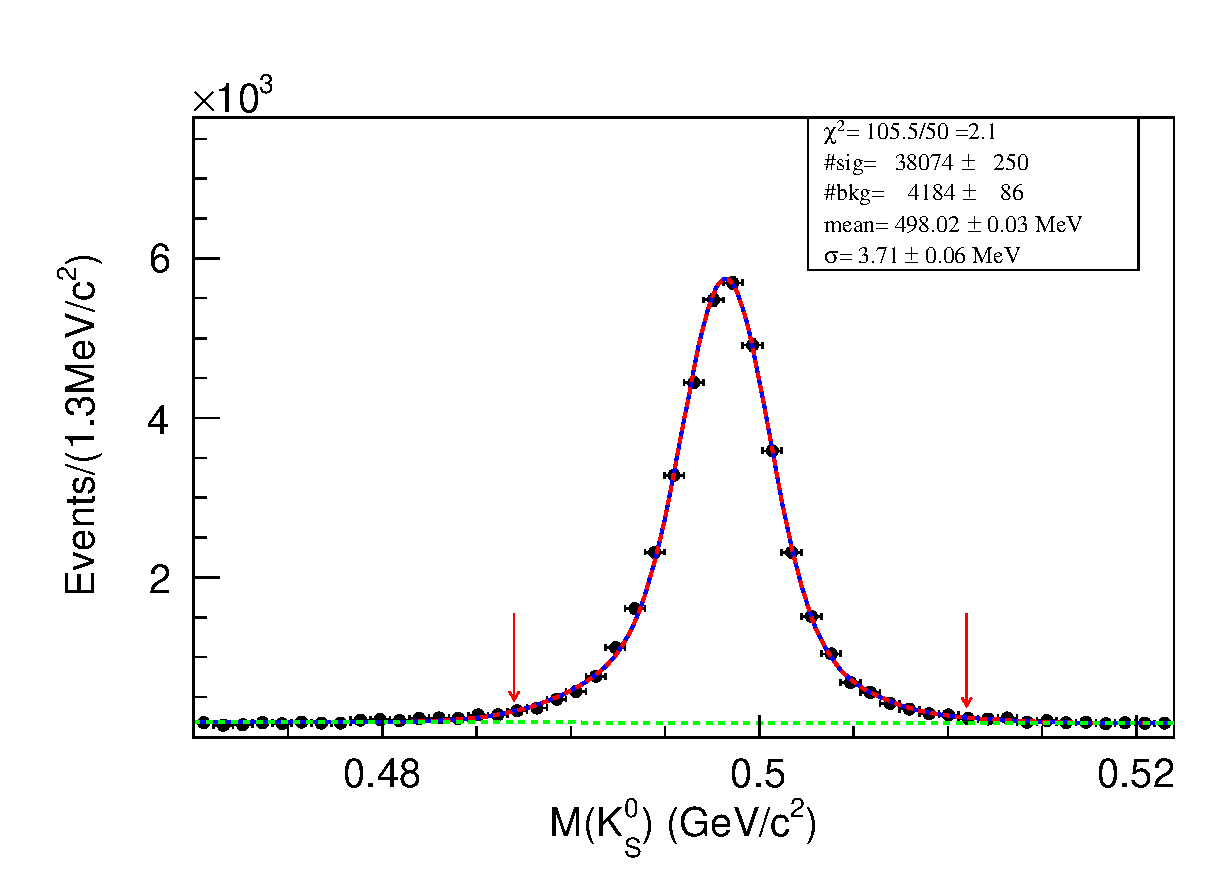
\includegraphics[width=0.8\linewidth]{dsToPPbar/mks.eps}
    \caption{$K_{S}^{0}$的不变质量谱}\label{fig:mks}
\end{figure}
\subsection{中性径迹的重建}
\label{sec:ds-neutral-track}
中性径迹指量能器所重建的电磁簇射,包含发生电磁簇射的位置及沉积能量的信息。实验上,光子会在量能器上沉积大部分能量、带电轻强子、
$K_{L}$和中子都
有一定的几率沉积少量的能量。我们主要的目标是重建光子。
对于用来重建 $\gamma$ 的中性径迹,我们有如下要求:
\begin{itemize}
    \item 在~EMC~桶部区域~($|\cos\theta| < 0.8$)~的沉积能量满足:$E > 25$ MeV;
\item 在~EMC~端盖区域~($0.86 < |\cos\theta| < 0.92$)~的沉积能量满足:
    $E > 50$MeV;
\item 径迹到达~EMC~的飞行时间满足:$0 \leqslant T \leqslant 14\,(\times 50 \,
    {\rm ns})$;
\item 与任何带电径迹在~EMC~上的沉积位置的距离大于~10~倍的标准偏差
    以排除带电径迹的带来的能量沉积。
\end{itemize}

\section{单标记分析}
按双标记方法的原则,我们首先重建一个$D_{s}^{-}$介子以做标记。我们选择单标记信号道的原则是产额大、本底低。我们经过比较选出了
三个最佳的标记道,它们是$K_{S}^{0} K^{-}$,$K^{+} K^{-} \pi^{-}$, 
$K_{S}^{0} K^{+} \pi^{-} \pi^{-}$。
\subsection{候选$D_{s}^{-}$}
以$K_{S}^{0}K^{-}$标记道为例来说明如何重建标记$D_{s}^{-}$介子。
首先按Sec.~\ref{sec:reconstruction}中叙述的方法
分别挑选出$K_{S}^{0}$和$K^{-}$所有的候选者。二者的所有组合都可能是
我们要寻找的$D_{s}^{-}$产物,我们用它们来推断$D_{s}^{-}$
运动学信息。每个事例我们只保留一个最佳的组合,也就是候选$D_{s}^{-}$,选取的原则的$M_{rec}(K_{S}^{0}K^{-})$最接近$m_{D^{*}_{s}}$,
其中$m_{D^{*}_{s}}$为$D^{*}_{s}$介子的不变质量,
\begin{equation}
    M_{rec}(K_{S}^{0}K^{-}) = \sqrt{{\left( \sqrt{s} 
       - E_{K_{S}^{0}} - E_{K^{-}} \right)}^{2}  - 
    {\left(\vec{p}_{K_{S}^{0}} + \vec{p}_{K^{-}} \right)}^{2}}.
\end{equation}
这个候选$D_{s}^{-}$被保留以做进一步分析。如果在单个事例中发现多个标记道
的候选,我们将全部保留并逐个处理。

\subsection{多重候选}
在单个事例中,对每个单标记道,我们只保留一个候选$D_{s}^{-}$粒子。为了能够有效
的挑选出正确的组合,我们选择$\Dsm$的反冲不变质量 ($M_{rec}(\Dsm)$)作为重要的
观测量。借鉴CELOc的经验~\cite{Alexander:2008aa},为了提高$M_{rec}(\Dsm)$的
分辨率,我们用如下公式计算$\Dsm$的能量
\begin{equation}
    E_{\Dsm} = \sqrt{m_{\Dsm}^{2} + |\vec{p_{\Dsm}}|^{2}},
\end{equation}
式中$m_{\Dsm}$为$\Dsm$的静止质量。相应的$M_{rec}(\Dsm)$可以写为
\begin{equation}
    M_{rec} \left( \Dsm \right)  =  \sqrt{%
        \left( E_{cm} - E_{\Dsm} \right){}^{2}
    - p_{\Dsm}^{2}  },
    \label{def:mrec}
\end{equation}
反冲不变质量$m_{rec}(\Dsm)$的分布如图~\ref{fig:recmassMC}所示,从$D^{*-}_{s}$
衰变出来的$\Dsm$介子的反冲不变质量为一个平台,但是从$e^{+}e^{-}$直接产生
$\Dsm$介子则会形成一个明显的峰结构,峰值恰好在$D_{s}^{*+}$的不变质量处。综合
考虑,我们选择$M_{rec}(\Dsm)$最接近$m_{D_{s}^{*+}}$的候选组合作为唯一的
$D_{s}^{-}$候选。

\subsection{单标记道的本底分析}
本底的主要来源包括:open charm和连续性本底。前者的$M_{rec}$不变质量远离信号
区,如图~\ref{fig:recmassMC}所示。为了压制这样的本底我们要求$D_{s}^{-}$的反
冲不变质量$M_{rec}$满足下列条件:
\begin{itemize} 
    \item $2.06 < M_{rec}(\Dsm) < 2.18 $ GeV $/c^{2}$ 
\end{itemize}

\begin{figure}[htbp]
    \centering
    \mbox{%
        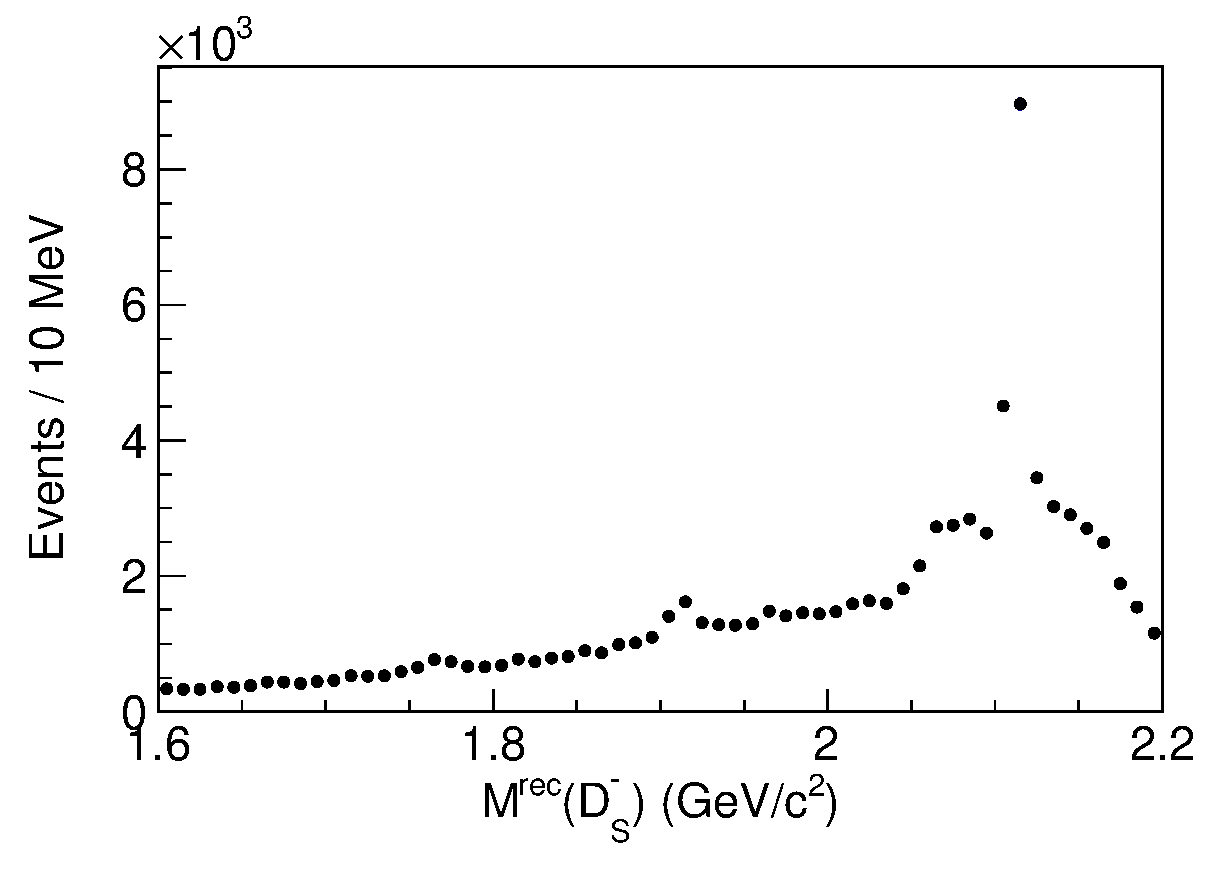
\includegraphics[width=0.8\linewidth]{dsToPPbar/recmass.eps}
    }
    \caption{标记$D_{s}^{-}$介子的反冲不变质量谱。
    }%
    \label{fig:recmassMC}
\end{figure}
此外,我们发现有一种主要的峰本底来自衰变$D^{*} \to D \pi$,由于从$D^{*}$衰变
出来的$\pi$介子动量很低,如图~\ref{Fig:pion_momentum}所示。
为了压低这个峰本底,我们要求$\pi$的动量大于100 MeV。
\begin{figure}[htbp]
    \centering
    \mbox{%
        \begin{overpic}[width=0.6\linewidth]{dsToPPbar/ppion.eps}
            %\put(50,70) {\color {green} {$ K^{+} K^{-} \pi ^{-} $}}
        \end{overpic}
    } 
    \caption{$\pi$介子的动量分布图。黑色的带误差棒的点代表数据,蓝色和红色
    的实线分别展示了$D_{s}^{*+}D_{s}^{-}$和$D^{*}D$蒙特卡洛样本中的动量分布。
    我们能发现一个明显由$D^{*}$衰变引起的峰结构。
    }\label{Fig:pion_momentum}
 \end{figure}
\subsubsection{峰本底}
在三个单标记道道中,只有$K_{S}^{0}K^{-}$由一种峰本底无法压制,这个峰本底
来自$D^{-}\to K_{S}^{0} \pi^{-}$,其中的$\pi^{-}$被误鉴别为$K^{-}$,不变质量
谱向右移动,从而形成峰本底。

\subsection{单标记产额和效率}

\subsubsection{拟合方法}
这些候选$D_{s}^{-}$既可能是我们需要的信号,也有可能为错误的组合(本底)。
信号事例和本底事例的不变质量谱形截然不同,
因此为了获得标记道的信号产额,我们把$D_{s}^{-}$的不变质量作为观察量。
我们决定采取极大似然法拟合$D_{s}^{-}$的不变质量分布来
获得信号产额。似然量的定义为
\begin{equation}
    L = e^{-N} \frac{N^{n}}{n!} 
    \prod_{i=1}^{i=N} \left( 
    \frac{n_{sig}}{n}  P_{sig}(m_{i}) 
    +  \frac{n_{bkg}}{n} P_{bkg}(m_{i})
\right),
\end{equation}
式中$N$,$n$ 分别为预期的总事例数和观测值, 
$n$为样本的中候选$D_{s}^{-}$个数,
$m_{i}$为第$i$个候选$D_{s}^{-}$的不变质量,
$P_{sig}$和$P_{bkg}$分别是信号和本底的概率
密度函数,
$n_{sig}$和$n_{bkg}$是同概率密度的参数分别指信号数和本底数。
拟合的过程也就是求似然函数极大值的过程,此时$n_{sig}$即为信号的产额。

\subsubsection{拟合模型的构造}
\begin{figure}[htbp]
    \mbox{%
        \begin{overpic} [width=0.45\linewidth] {dsToPPbar/Ds_mc401.eps}
            \put(80, 55){\color{blue} {(1)} }
        \end{overpic}

        \begin{overpic} [width=0.45\linewidth] {dsToPPbar/Ds_mc400.eps} 
            \put(80, 55){\color{blue} {(2)} }
        \end{overpic}

    }
        \begin{overpic} [width=0.45\linewidth]{dsToPPbar/Ds_mc406.eps} 
            \put(80, 55){\color{blue} {(3)} }
        \end{overpic}

    \caption{标记侧的$M(D_{s}^{-})$分布及拟合结果。
        数据是带误差棒的黑色点。标记道分别是 (1)
        $K^{+}K^{-}\pi^{-}$ (2) $ K_{S}^{0} K^{-}$ 
        (3)$ K_{S}^{0} K^{+}\pi^{-}\pi^{-}$.
    }\label{Background_analysis_for_ST_modes}
\end{figure}
图\ref{Background_analysis_for_ST_modes}是数据和蒙特卡洛样本之间的对比,从图中我们
可以看出蒙特卡洛模拟的足够好,除了单标记道$K_{S}^{0}K^{-}$以外,均没有明显的峰状
本底。因此我们用切比雪夫多项式描述本底的形状。我们尝试用双高斯分部描述MC
中信号的形状,为了补偿数据和蒙特卡洛样本之间的分辨率差异,我们把经高斯函数卷积后的
信号蒙特卡洛样本的形状描述数据中的信号形状,其中的高斯函数的中心值和分辨作为自由参数
由数据决定。
\subsection{拟合结果}
\begin{figure}[htpb]
    \centering
    \mbox{%
        \begin{overpic}[width=0.45\linewidth]{dsToPPbar/Ds401.eps}
            \put(30, 50){\color{blue} {(1)}}
        \end{overpic}
        \begin{overpic}[width=0.45\linewidth]{dsToPPbar/Ds400.eps}
            \put(30, 50){\color{blue} {(2)}}
        \end{overpic} 
    }
        \begin{overpic}[width=0.45\linewidth]{dsToPPbar/Ds406.eps}
            \put(30 ,50) {\color{blue} {(3)} }
        \end{overpic}
    \caption{%
        不同标记道中的$D_{s}^{-}$不变质量谱的拟合结果。
        三个标记道分别是 (1) $K^{+}K^{-}\pi^{-}$ 
        (2) $K_{s}K^{-}$ (3) $K_{S} K^{+}\pi^{-}\pi^{-}$。 
        红色的点虚线是峰本底的贡献。
    }%
    \label{fig:ST_data_fit}
\end{figure}
效率的定义为
\begin{equation}%
    \label{eq:ST-efficiency}
    \epsilon = \frac{N^{ST}}{N^{generated}}
\end{equation}
式中$N^{ST}$是标记$D_{s}^{-}$的产额,$N^{generated}$则是样本中
该标记$D_{s}^{-}$ 总数目。拟合的结果如图\ref{fig:ST_data_fit},相关
的效率在表\ref{table:ST_yield_and_efficiency}做了汇总。
\begin{table}[htbp]
    \centering
    \begin{tabular}{l l c c c c}
        \toprule[0.2em]
        标记道 ($\alpha$) & 次级衰变 & 产额 (MC) & 总数 & $\epsilon^{ST}(\%)$ &
        产额 (data)
        \\     
        \midrule
        $D_{s}^{-}\rightarrow K^{+}K^{-}\pi^{-} $ &-
        & 2642391 $\pm$ 2455 & 6243628 &    42.32    $\pm$    0.04      &  140277$\pm$ 635
        \\  

        $D_{s}^{-}\rightarrow K_{s}K^{-} $ & $K_{S}^{0}\rightarrow \pi^{+}\pi^{-}$ 
        & 565897 $\pm$ 2025 &     1147161     &    49.33    $\pm$    0.18  & 31267 $\pm$ 261
        \\ 

        $D_{s}^{-}\rightarrow K_{s}K^{+}\pi^{-}\pi^{-} $ & $K_{S}^{0} \rightarrow \pi^{+}\pi^{-} $ 
        & 272531 $\pm$ 925 &    923848    &    21.08    $\pm$    0.07  & 14547
        $\pm$ 214 \\
        \bottomrule
    \end{tabular}
    \caption{单标记效率及数据中各个标记道产额。
    }\label{table:ST_yield_and_efficiency}
\end{table}

\section{信号道的重建}\label{Double-Tag}
\subsection{信号挑选}
信号侧的$D_{s}^{+}$介子衰变到$p\bar{p}e^{+}\nu_{e}$。
如前文讨论,电子由于动量过低而难以被重建,因此重要的信号是发现正反
质子对,能够发现电子作为一个辅助手段。当电子恰好被完整重建时,我们
重建这个电子作为压低本底的一个手段。
基于信号蒙特卡洛样本,本文首先详细研究了电子被重建的几率。图\ref{Fig:tracks}
展示了信号蒙特卡洛样本中标记一个$D_{s}^{-}$之后剩余的带电径迹数目的分布,
我们发现发现三条径迹的情况仅仅占6.8\%,这意味着至少有93\%以上的电子
丢失了。
\begin{figure}[htbp]
    \centering
    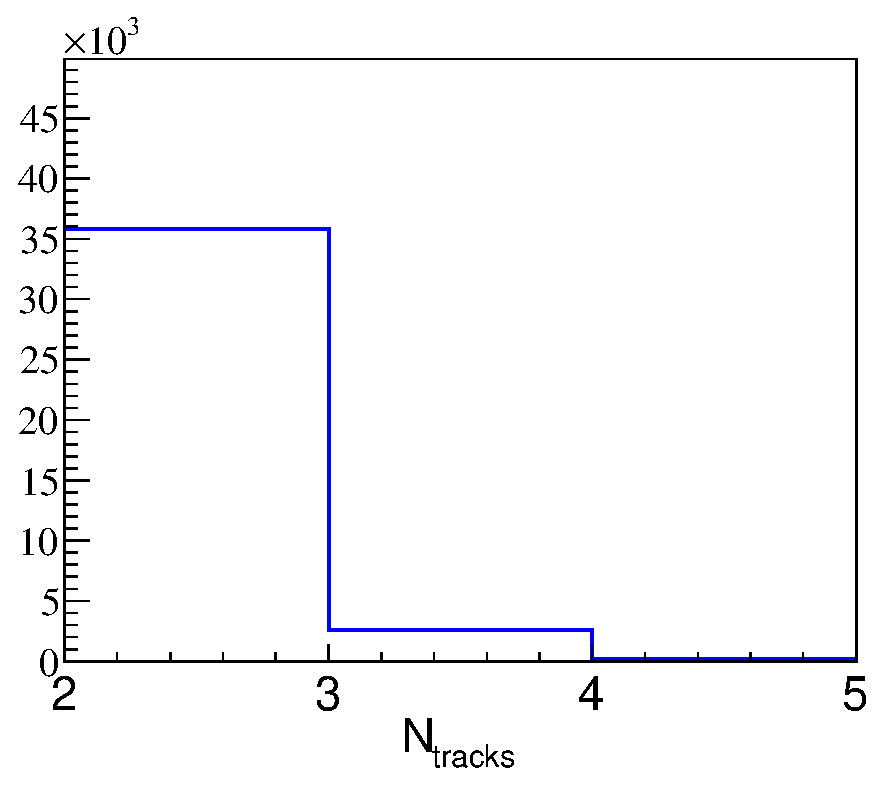
\includegraphics[width = 8 cm]{dsToPPbar/Tracks_signalMC.eps}
    \caption{信号蒙特卡洛样本中的带电径迹数目(除了标记侧)分布。
    }\label{Fig:tracks}
\end{figure}
因此我们按带电径迹个数把样本分为两类:
\begin{itemize}
    \item \textbf{A}: 仅有两条带电径迹,并且被鉴别为正反质子对
    \item \textbf{B}:有三条带电径迹,其中有一对带电径迹被鉴别为正反质子对
\end{itemize}
我们将在下文里对两种情况分别进行讨论。

\subsubsection{进一步讨论}
\subsubsection{质子和电子的动量信息}
在带电粒子中,质子的MDC中的电离能损最大。在BESIII的探测器上,动量低于
200MeV$/c$的质子,其径迹不可能被重建。因此图中\ref{Fig:momenta_of_proton},
质子的动量谱在220MeV$/c$附近急剧下降。但是仍有少数事例存在误鉴别的质子,
造成动量谱在200MeV$/c$以下不为0,故而,为了压低本底,我们要求质子的
动量大于200MeV$/c$。
\begin{figure}[htbp]
    \centering
    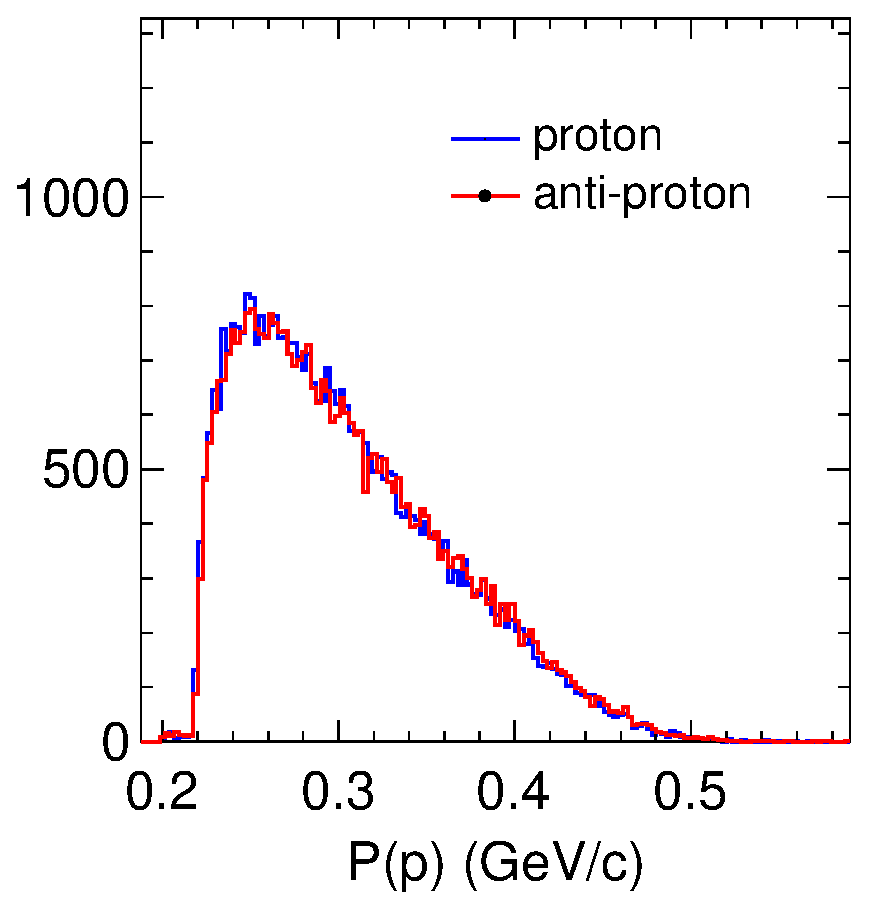
\includegraphics[width = 8 cm]{dsToPPbar/Momentum_proton_signalMC.eps}
    \caption{信号蒙特卡洛样本中正反质子对的动量分布。红色和蓝色的实线分别代表质子和
    反质子。
    }\label{Fig:momenta_of_proton}
\end{figure}
另一方面,由于相空间的限制,电子的动量低于90MeV$/c$,在情况\textbf{B},我们
能清晰地把质子和电子区分开,不必对电子做任何粒子鉴别。如图\ref{Fig:pele}
所示,在遍举蒙特卡洛样本中存在其他粒子被误作为电子,本文根据它们之间的动量分布
的不同,对电子的动量做要求能显著的压低这种本底。

类似的,本文定义了\textbf{FOM}来优化电子的选择条件,\textbf{FOM}的定义为
\begin{equation}
    FOM = \frac{S}{\sqrt{B}}, 
    \label{eq:FOM-ele}
\end{equation}
式中$S$和$B$分别是信号数和本底个数,其中$S$从信号
蒙特卡洛样本中得到,$B$则在混合蒙特卡洛样本中取得。

从\textbf{FOM}~\ref{Fig:pele}的曲线可以看出,
\textbf{FOM}的值大致在90MeV
达到峰值,这几乎也是电子动量大小的运动学
极限 (\ref{Equ:cut_on_momentum_of_electron}),综合考虑,我们要求 
重建出的电子动量不得大于90MeV. 
\begin{figure}[htbp]
    \centering
    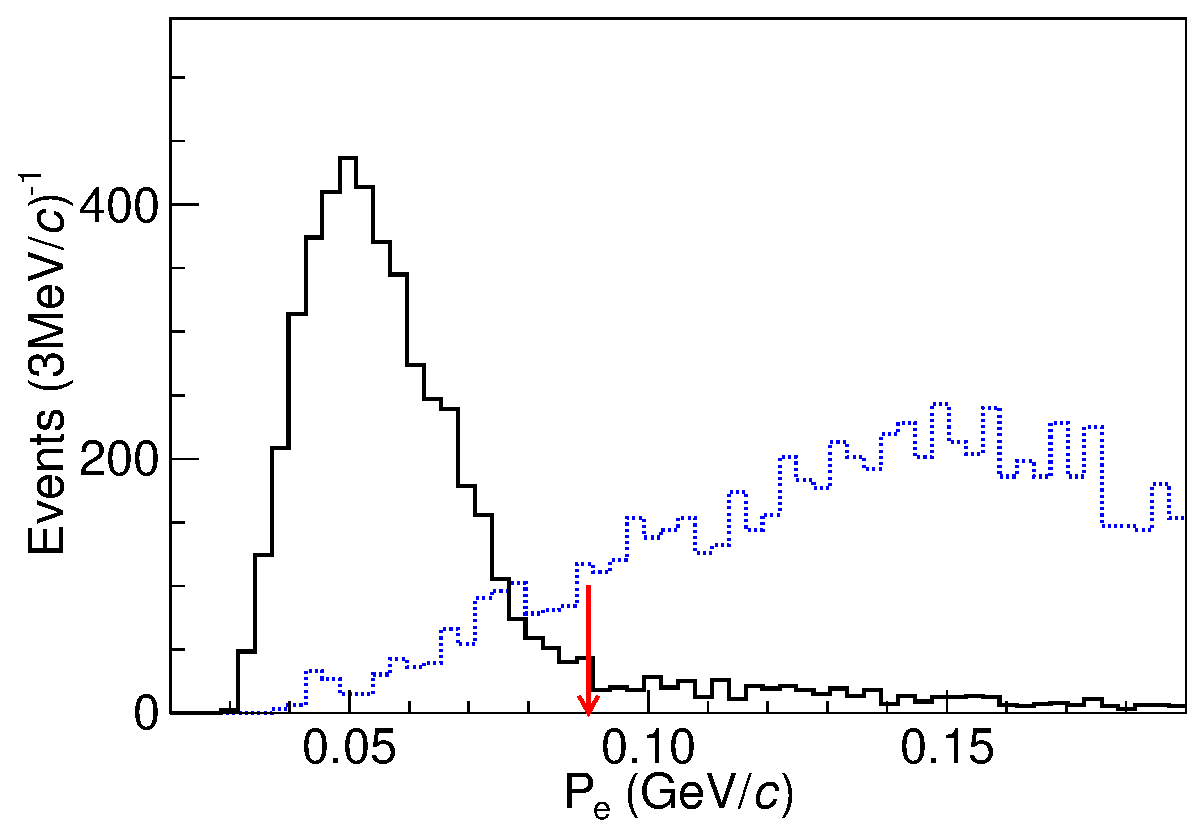
\includegraphics[width = 0.45\linewidth]{dsToPPbar/pele.eps}
    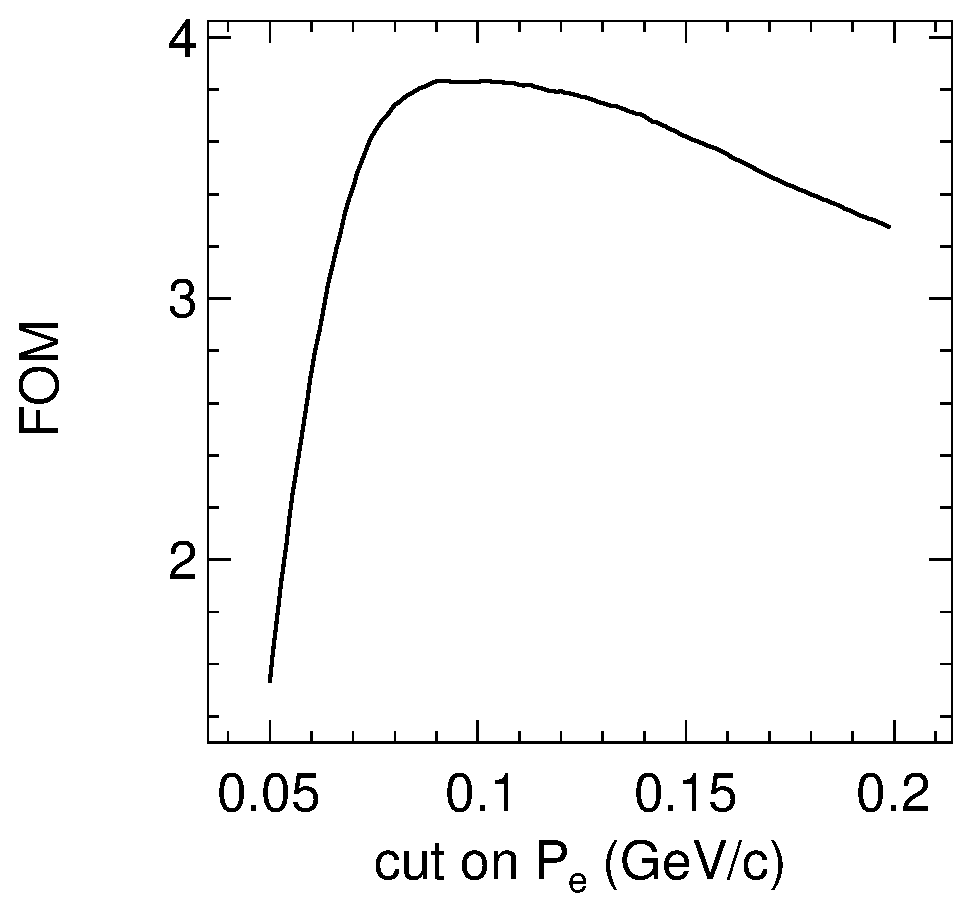
\includegraphics[width = 0.45\linewidth]{dsToPPbar/Optimiz_cut_Pele.eps}
    \caption{左图:电子的动量分部。绿色的实线表示信号形状,
    而蓝色的虚线表示本底的形状。右图: \textbf{FOM}曲线。
    }%
    \label{Fig:pele}
\end{figure}

\subsubsection{$MM^{2}$}
由于半轻道中中微子不能被BESIII探测器重建,因此丢失不变质量常常作为
重要的观测量以此得到中微子的产额。然而在本分析中,除了中微子,90\%
以上的电子也由于难以被探测而丢失,使得丢在不变质量不再是理想的观测量。
然而质子对的存在恰能够推测出电子的存在,根据轻子数守恒,必然存在一个电子
型中微子。这就是本文之所以仅仅把丢失不变质量作为压低本底的手段,而不是
决定信号产额的观测量。本文分两种情况,即是否找到了电子径迹,分别定义了
丢失不变质量,具体的定义见式.~\ref{eq:MM_define}
\begin{equation}
    \begin{aligned}
        \label{eq:MM_define}
        \textbf{2 tracks}: 
        MM^{2} &= {\left( E_{cm} -  E_{ST} - E_{p} - E_{\bar{p}} \right)}^{2} 
        -{\left( p_{p} + p_{\bar{p}} \right) }^{2} 
        \notag \\
        \textbf{2 tracks}:
        MM^{2} &= {\left( E_{cm} -  E_{ST} -E_{p} -E_{\bar{p}} - E_{e}
        \right)} ^{2} - {\left(p_{p} + p_{\bar{p}}  + p_{e} \right)}^{2}
    \end{aligned}
\end{equation}
式中$E_{ST}$ 和 $p_{ST}$ 分别是$e^{+}e^{-}$质心系下标记$\Dsm$的总能量和
总动量,$E_{p}$, $E_{\bar{p}}$,$p_{p}$,和 $p_{\bar{p}}$ 
分别是正反质子相应的能量和动量,$E_{e}$ and $p_{e}$ 分别是电子的能量和动量,
只有在情况\textbf{B}下,我们才在计算$MM^{2}$时计入电子的能量
和动量信息。
如图所示\ref{fig:MMbkg},对于不同的标记道,$MM^{2}$的本底形状大致相同,
峰值均在0.0 ${(GeV/c^{2})}^{2}$, 位于信号的左侧。
\begin{figure}[htbp]
    \begin{center}
    \mbox{%
        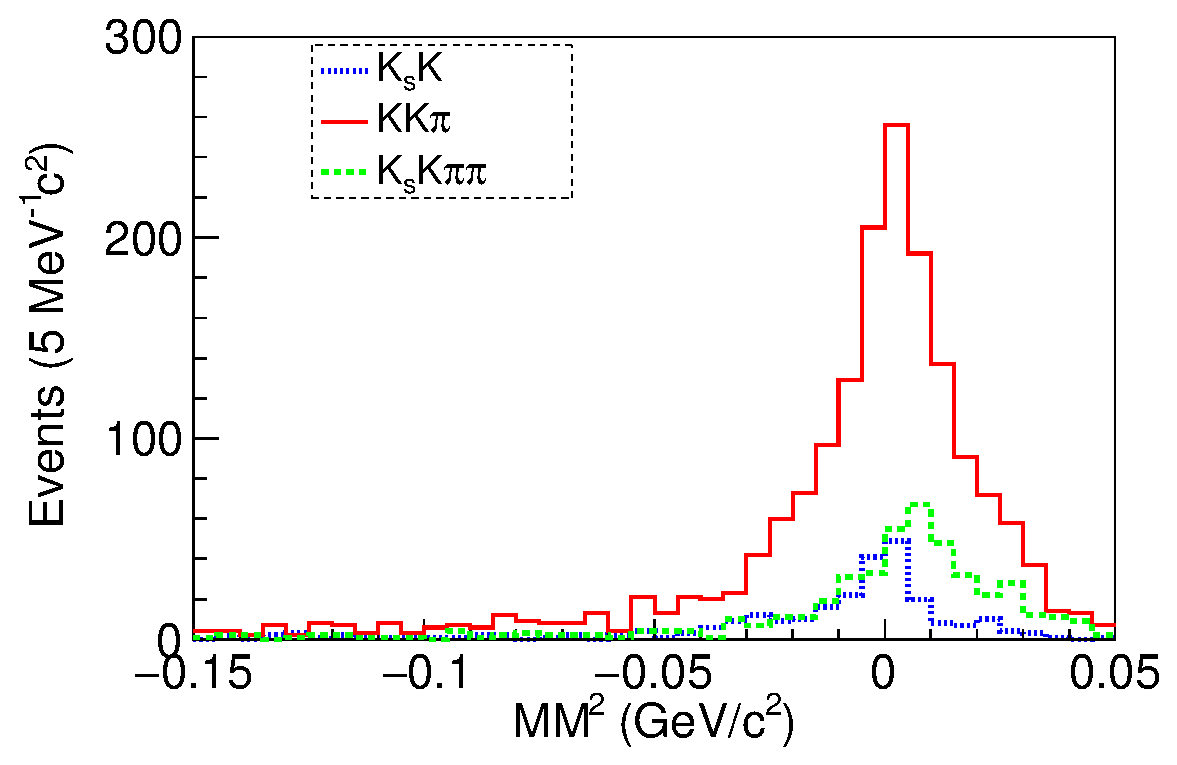
\includegraphics[width = 0.8\linewidth]{dsToPPbar/MMbkg.eps}
    }
    \end{center}
    \caption{$q\bar{q}$样本中$MM^{2}$的分布。红色、蓝色和绿色的实线分别表示
    三个标记道:
    $KK\pi$,$K_{S}^{0}K$ and $K_{S}^{0}K^{-}\pi^{+}\pi^{+}$
    }\label{fig:MMbkg}
\end{figure}

\begin{figure}[htbp]
    \centering
    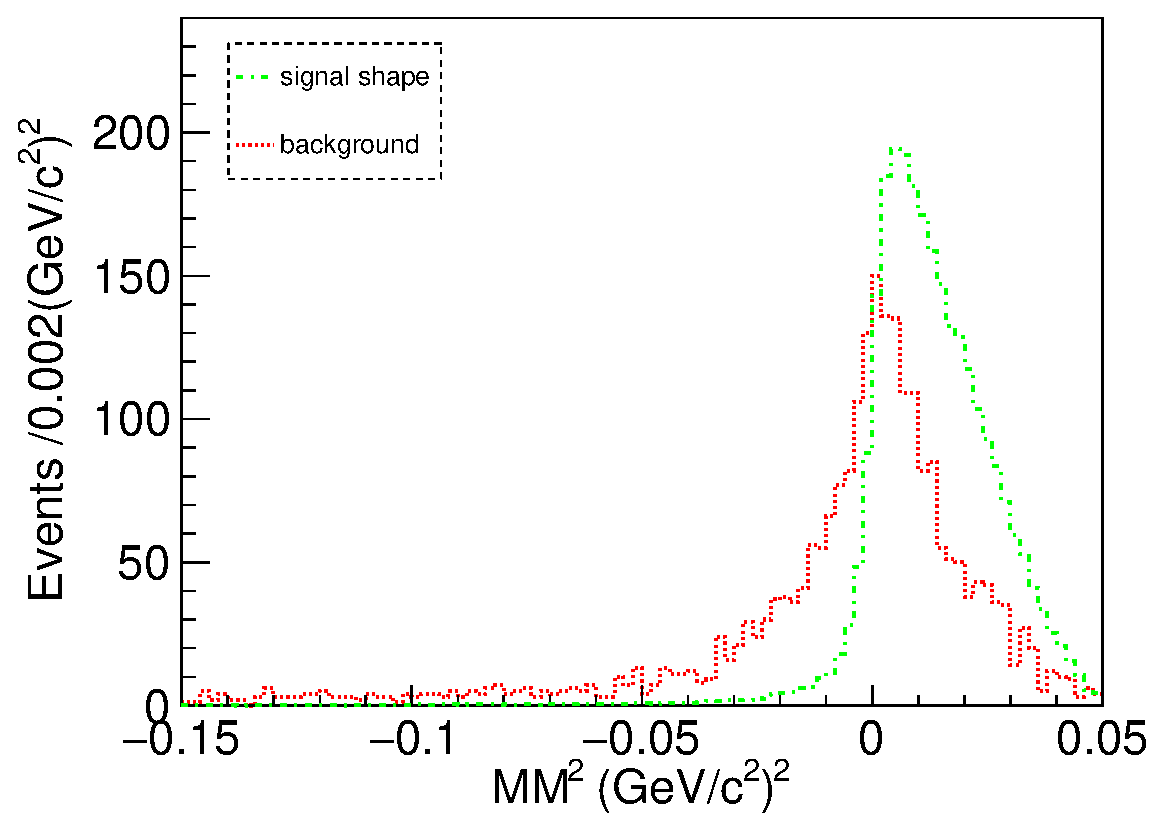
\includegraphics[width = 0.8\linewidth]{dsToPPbar/MC_Sig_compare.eps}
    \caption{合并所有的标记道之后的$MM^{2}$分部。绿色和红色的实线分别
    表示信号和本底的形状。
    }\label{fig:MC_Sig_compare}
\end{figure}
为了研究信号模型对$MM^{2}$的影响,近而确定对$MM^{2}$的要求,我们产生了
两种信号蒙特卡洛样本,得到的$MM^{2}$的形状如图\ref{fig:MM_model}所示。综合考虑
\textbf{FOM}和潜在的系统误差,一方面,如图\ref{fig:FOM}在0.0
${(GeV/c^{2})}^{2}$达到最大值,另一方面,$MM^{2}$ 在大于0.0 
${(GeV/c^{2})}^{2}$区域内形状的不确定性很高,若选择条件右移,会造成
潜在的系统误差。因此本文要求$MM^{2} >0.0{(GeV/c^{2})}^{2}$,后续的研究表明
这个选择条件带来的误差仅仅为1\%。
\begin{figure}[htbp]
    \begin{center}
    \mbox{%
        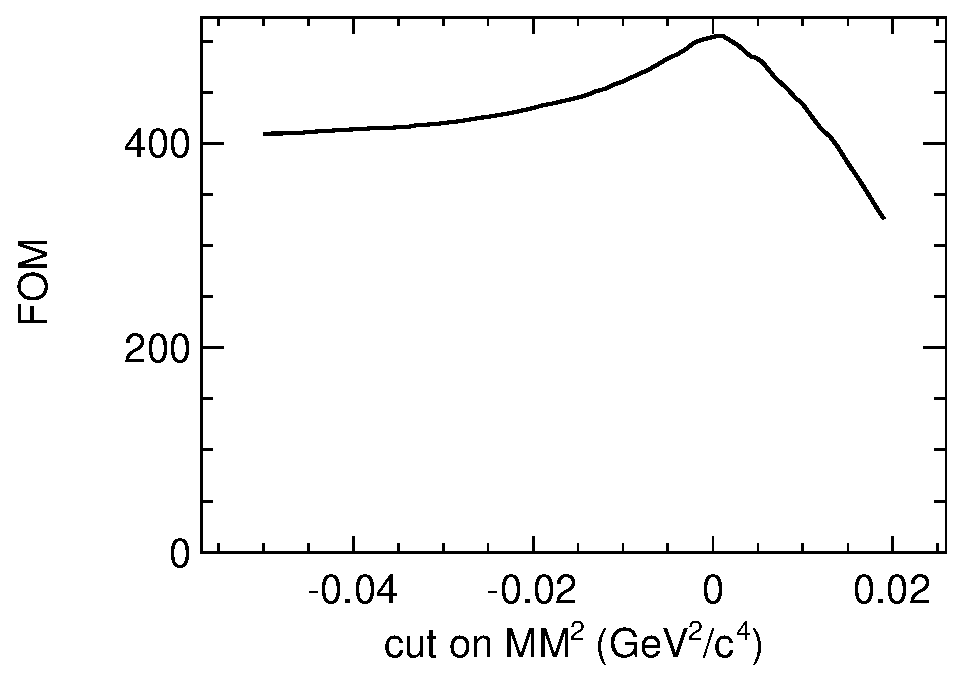
\includegraphics[width = 0.9 \linewidth]{dsToPPbar/Optimiz.eps}
    }
    \end{center}
    \caption{变动对$MM^{2}$的要求。阈值在$0.0 GeV/c^{2}$附近\textbf{FOM}
    达到极大值。
    }\label{fig:FOM}
\end{figure}
\begin{figure}[htbp]% different model
    \centering
    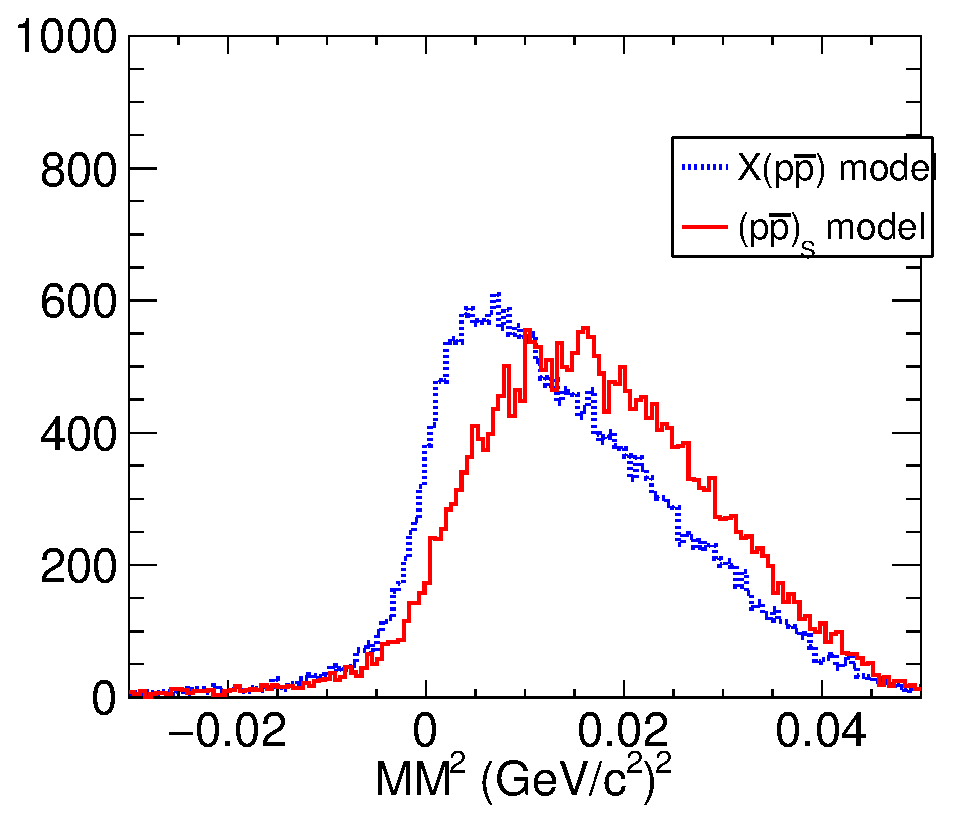
\includegraphics[width=0.9 \linewidth]{dsToPPbar/MMsig.eps}
    \caption{蓝线和红线分别表示模型${(p\bar{p})}_{S}$和$X(p\bar{p})$中
    的信号形状。
    }\label{fig:MM_model}
\end{figure}

\subsubsection{本底分析}
本底的分析过程是基于35倍于数据亮度的混合蒙特卡洛样本。本底的主要来源是$q\bar{q}$
过程,原因是其能产生丰富的正反质子对。从不变质量谱\ref{fig:qq_bkg}上
可以看出没有明显的峰状本底。其他过程中,我们只发现几个open charm过程,
这是由于质子的误鉴别率比较低。对于我们最关心的$D_{s}^{*}D_{s}$过程,
只有3个事例通过了事例挑选程序,从而可以推断出数据中的峰本底要少于0.1个,
这是完全可以忽略不计。
\begin{figure}[htbp]
    \begin{center}
        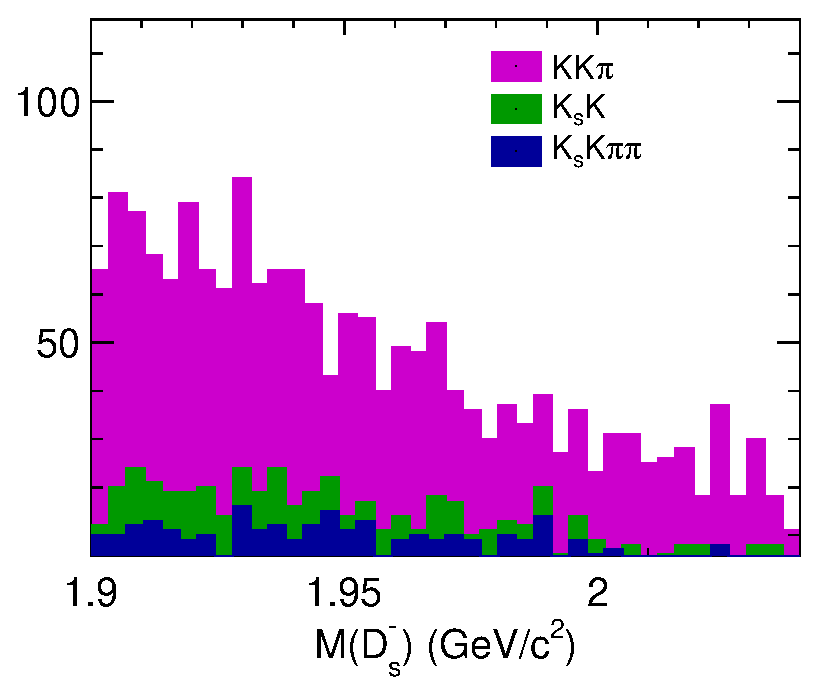
\includegraphics[width=8cm]{dsToPPbar/tag_mass.eps}
    \end{center}
    \caption{$q\bar{q}$样本中的$M(D_{s}^{-})$分布。红色、绿色和蓝色
    的实线分别展示标记道$KK\pi$、$K_{s}K$和
    $K_{s} K^{+} \pi^{-}\pi^{-}$中的不变质量谱。
    }\label{fig:qq_bkg}
\end{figure}
在最大的本底来源--$q\bar{q}$ 中,几种典型的过程为
$e^{+}e^{-} \rightarrow p \bar{p} 4\pi$, 
$p \bar{p} K^{+} K^{-} 2\pi n\pi^{0}$ ($n=0,1,2\cdots$)。前者由于
其中一个$\pi$介子 被误鉴别为$K$介子并和其他的$\pi$介子
误组合成一个$D_{s}^{+}$, 后者则是$K$介子和$\pi$介子直接误组合
成一个$D_{s}^{+}$。
图~\ref{Fig:different_background}则显示这几种典型本底的形状较为相似,
因此我们直接用混合蒙特卡洛样本中的本底形状来描述本底,而把这些典型过程中的本底
形状的细微差异作为一项系统误差来源。

\begin{figure}[htbp]
    \mbox{%
        \begin{overpic}[width = 0.45 \linewidth]{dsToPPbar/Mds_qq_401.eps}
            \put(25,55) {\scalebox{0.7}{$K^{+} K^{-} \pi^{-}$}}
        \end{overpic}

        \begin{overpic}[width = 0.45 \linewidth]{dsToPPbar/Mds_qq_400.eps}
            \put(25,55) {\scalebox{0.7} {$K^{-} K_{s}^{0}$}}
        \end{overpic}
    }
    \mbox{%
        \begin{overpic}[width = 0.45 \linewidth]{dsToPPbar/Mds_qq_406.eps}
            \put(25,55) {\scalebox{0.7}{{$ K_{s}^{0} K^{+} \pi^{-} \pi^{-} $} }}
        \end{overpic}
    }

    \caption{来自几种主要本底信号道中的本底形状。
    }%
    \label{Fig:different_background}
\end{figure}

\subsubsection{双标记效率}%
\label{sec:dt-efficiency}
为了拿到双标记的效率,我们产生了一千万的信号蒙特卡洛样本。在这些样本中,有一个
$\Ds$介子衰变到所有已知的衰变道,另一个$\Ds$介子衰变到信号道。与单标记侧的
分析类似,我们通过拟合标记$\Ds$的不变质量谱来得到信号的产额。
在拟合的过程中,我们借助于工具\textbf{RooKeyPdf}从信号蒙特卡洛样本中直接获取信号形状,
用二阶切比雪夫多项式来描述本底的形状。图\ref{Fig:DT}展示了拟合的结果,
表\ref{table:DT_yield_and_efficiency}中是双标记的产额和效率
\begin{table}[htpb]
    \caption{双标记的产额和效率DT。$\epsilon_{1}$和$\epsilon_{2}$分别表示
    来自模型$X(p\bar{p})$和${(p\bar{p})}_S$的效率。
    }\label{table:DT_yield_and_efficiency}
    \centering 
    \begin{tabular}{lcccc} 
        \toprule
        衰变模式 &  样本大小(事例数)  &  $\epsilon^{ST} (\%)$ & 
        $\epsilon ^{DT}_{1} /\epsilon^{ST}(\%)$  & $\epsilon^{DT}_{2} / \epsilon^{ST} (\%)$
        \\  
        \midrule
        $D_{s}^{-} \rightarrow K^{+} K^{-} \pi^{-}$ & 500000 & $
        42.32 \pm 0.04 $ & $ 16.8 \pm 0.1 $  & $20.4 \pm 0.1$\\
        %16.77
        $D_{s}^{-} \rightarrow K^{-} K_{s}^{0}$ & 500000 &$ 49.33
        \pm 0.18 $ & $ 16.0  \pm 0.1 $ & $19. 5 \pm 0.1$\\

        $D_{s}^{-} \rightarrow K_{s}^{0} K^{+} \pi^{-} \pi^{-} $ &
        500000 &$ 21.08 \pm 0.07 $ & $ 14.8 \pm 0.2$  & $18.1 \pm
        0.2$\\
        \bottomrule
    \end{tabular}
\end{table}

\begin{figure}[htbp]
    \mbox{%
        \begin{overpic}[width = 0.32 \linewidth]{dsToPPbar/Ds401_x1835.eps}
            \put(20,75) {\scalebox{0.7}{$K^{+} K^{-} \pi^{-}$}}
        \end{overpic}

        \begin{overpic}[width = 0.32 \linewidth]{dsToPPbar/Ds400_x1835.eps}
            \put(20,75) {\scalebox{0.7} {$K^{-} K_{s}^{0}$}}
        \end{overpic}

        \begin{overpic}[width = 0.32 \linewidth]{dsToPPbar/Ds406_x1835.eps}
            \put(20,75) {\scalebox{0.7}{{$ K_{s}^{0} K^{+} \pi^{-} \pi^{-} $} }}
        \end{overpic}
    }
    \caption{对信号蒙特卡洛样本中$D_{s}^{-}$不变质量谱的拟合结果。
    黑色的带误差棒的点代表数据,
    蓝色、绿色和红色的线分别表示拟合结果、信号形状和本底形状。
    }\label{Fig:DT}
\end{figure}

\subsubsection{效率修正}%
\label{Sec:Correction_of_Efficiency}
由于低动量的质子和物质(这里指探测器)的相互作用比较复杂,蒙特卡洛模拟和真实
的相互作用有些差异,因此本文利用控制样本首先得到数据和蒙特卡洛样本之间的效率差异,
并进一步修正了双标记的效率。
由于粲介子几乎不衰变到质子,因此本文从$q\bar{q}$过程中选择控制样本,最为
合适的一个样本是 
$e^{+} e^{-} \rightarrow p \bar{p} \pi^{+}\pi^{-}$,具有本底低、样本大的优点。
本文利用这个控制样本做了质子鉴别的系统研究,相关的细节见附录。

本文用观测量$\Delta \epsilon$(\ref{Equ:correct_PID}) 来衡量数据
之间蒙特卡洛样本效率差异
\begin{equation}
    \label{Equ:correct_PID}
    \Delta \epsilon =\left( \frac{\epsilon_{data} }{\epsilon_{MC}} 
        -1 \right) \times 100\%
\end{equation}
式中$\epsilon_{Data}$ 和 $\epsilon_{MC}$分别是数据和蒙特卡洛样本中的质子鉴别效率。

由于质子的粒子鉴别效率依赖于动量大小以及飞行方向,因此本文按质子的动量和
极角划分来获取动量。第$i$个区间内的效率记做$\epsilon_{i}$,
相应的差异记做$\Delta \epsilon_{i}$。
本文这里定义了修正因子$\delta$来衡量总体的效率修正
\begin{equation}
    \delta = \frac{\epsilon^{cor}}{\epsilon^{old}} -1   
    \label{eq:corr-factor}
\end{equation}
式中$\epsilon^{old}$为信号样本中修正之间的总体效率,
$\epsilon^{cor}$是同样的样本中经过效率修正之后的总体效率。
接下来将讨论效率修正的细节。在第$i$的区间内,修正的效率为
\begin{equation}
    \epsilon^{cor}_{i} = \epsilon_{i} \cdot (1+ \Delta \epsilon_{i}) \notag
\end{equation}
对所有的区间求平均后,很容易就得到总体的效率(\ref{eq:average_efficiency}),
\begin{equation}
    \label{eq:average_efficiency}
    \begin{aligned}
        \epsilon^{cor} &= \sum _{i} \frac{n_{i}}{N} \cdot
        \epsilon^{cor}_{i} \notag \\
        &= \sum_{i} \frac{n_{i}^{obs} \cdot (1+ \Delta \epsilon_{i}) }{N} 
    \end{aligned}
\end{equation}
式中$N$是信号样本中的总信号数,
$n_{i}$是信号样本中第$i$个区间内的事例数,$n^{obs}_{i}$则是经过
事例挑选程序后的第$i$个区间内的信号产额,
$\Delta \epsilon_{i}$ 是从控制样本中得到的效率差异。

利用上式,很容易得到效率修正因子$\delta$(\ref{eq:correct_factor}),
\begin{equation}
    \label{eq:correct_factor}
    \delta  = \sum_{i} \frac{n_{i}^{obs} \cdot (1+ \Delta
\epsilon_{i})}{N^{obs}} -1 
\end{equation}
式中$N^{obs}$信号蒙特卡洛样本中通过事例挑选程序的总事例数。
把质子样本按动量大小进行划分,间距设为50MeV,以此得到修正因子的大小为:
 \begin{equation}
     \delta = (-0.9 \pm 2.2)\% \notag 
 \end{equation}
为保守起见,我们把系统误差设为$2.7\%$。

\subsection{获取分支比的策略研究}
在信号模型中,$X(p\bar{p})$的质量和宽度分别是$1.834$GeV、$68$MeV。
重建后的$p\bar{p}$不变质量谱如图\ref{fig:mPP}所示,
由于正反质子对的质量和比的$X(p\bar{p})$质量还要小,
因此这里不能看到$X(p\bar{p})$完整形状,
只能看到其尾巴。另一方面,由于探测的效率随质子的动量变化而急剧变化,
可以看到$X(p\bar{p})$的重建之后线型发生了极大的变化。
为了避免这种不确定性,一种可行的方案是只做一维的拟合来获得信号数,这个
观测量只能是标记$\Dsm$的不变质量,而不能是$M(p\bar{p})$或$MM^{2}$。
这里要求$M(p\bar{p})$在信号区$[1.87,1.97] {(GeV/c^{2})}^{2}$。
为了充分利用标记道的信息,本文使用联合拟合方案。
联合拟合的似然值定义为
\begin{eqnarray}
    \mathcal{L}^{\alpha} = \frac{e^{- (N_{\rm sig}^{\alpha} + N_{\rm
    bkg}^{\alpha})}}{n^{\alpha}!}
    % \prod_{i=0}^{n^{\alpha}}
     \prod_{i=1}^{n^{\alpha}}
    \left( N_{\rm sig}^{\alpha} P_{\rm sig}^{\alpha}(M_{D_{s}^{-}})
    + N_{\rm bkg}^{\alpha} P_{\rm bkg}^{\alpha}
    \left(M_{D_{s}^{-}}\right) \right),
\end{eqnarray}
式中 $n^{\alpha} = N_{\rm sig}^{\alpha} + N_{\rm bkg}^{\alpha}$ 是双标记的
观测到的总事例,$i$代表第$i$个事例,$N_{\rm sig}^{\alpha}$和$N_{\rm
bkg}^{\alpha}$代表待拟合的信号数和本底数,
$P_{\rm sig}^{\alpha}$和$P_{\rm bkg}^{\alpha}$分别是标记道$\alpha$的
信号和本底的概率密度函数。这三个标记道的似然值拥有一个共同的参数,
这个参数就是信号道的分支比,故而能最大的利用数据的信息。
\begin{figure}[htbp]
    \centering
    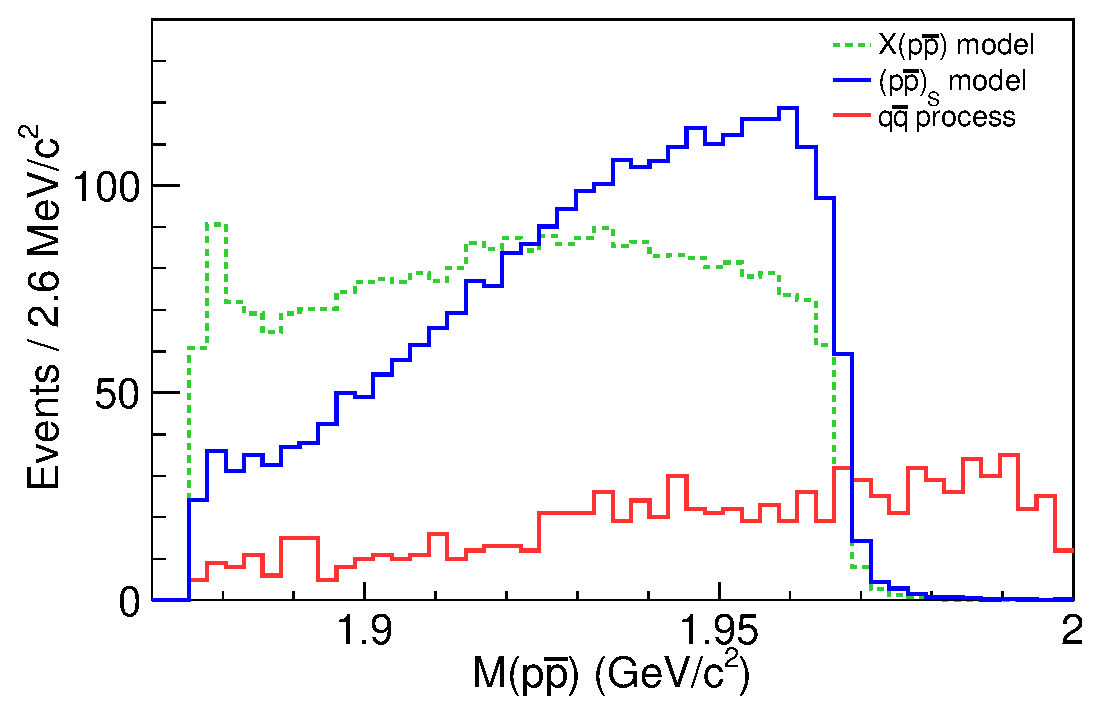
\includegraphics[width = 0.8 \linewidth]{dsToPPbar/mPP.eps}
    \caption{正反质子对的不变质量谱。
    绿色和红色的实线分别是信号和本底的形状。
    }\label{fig:mPP}
\end{figure}
如果在数据中的信号显著性小于3$\sigma$,本文则会为这个衰变道设一个上限。

\subsection{输入输出检查}
在正式分析真实的数据之间,做输入输出的检查是必要的。考虑到数据中只能
出现两种情况,要么有明显的信号,要么没有,因此本节分两种情况做检查,
首先考虑到可能看到信号,本文选择先从遍举 蒙特卡洛样本中随机抽样出和数据量
等同的子样本,并混入适当的信号蒙特卡洛样本,以此做输入输出检查。之后在遍举
MC子样本中不放任何信号,来研究实验的灵敏度。

\subsection{分支比的输入输出检查}
如上节所述,我们将把适当的信号蒙特卡洛样本混入遍举 MC之中来做分支比的
输入输出检查。信号道的分支比设为0.1\%,并利用\textbf{TRandom}从信号样本
中随机抽取相应个数的事例。类似的,
我们从混合样本中随机抽取与真实数据等大小的子样本。之后,利用同时拟合技术
去拟合上述操作得到的伪数据样本来获取分支比。更改随机数种子,重复以上操作,
便可以得到一系列的结果。
这这些结果中,某次的拟合结果如图~\ref{fig:total_fitting}示意。
实验上常常采取观察量\textbf{PULL}来衡量输入输出检查的好坏。若\textbf{PULL}
的中心值偏离0则意味了输出值有一定的偏差。
式\ref{eq:pull}定义了$\textbf{PULL}$,
\begin{equation}
    \label{eq:pull}
    PULL = \frac{\mu^{obs} -\mu_{0}}{\sigma_{\mu}^{obs}}
\end{equation}
式中$\mu^{obs}$和$\sigma_{\mu}^{obs}$分别是每次测量结果的中心值和误差,
$\mu_{0}$是输入值。在本节的输入输出检查中,$\mu$对应于信号
$D_{s}^{+} \to p\bar{p} e^{+} \nu_{e}$的分支比,$\mu_{0}$的取值是0.1\%。
本节多次实验得到的\textbf{PULL}分布如图\ref{Fig:pull_distribution}
所示。为了检验无偏性,这里用正态分布去拟合这个pull分布,拟合
结果见图\ref{Fig:pull_distribution},可以看出拟合结果没有明显的偏差。

\begin{figure}[htbp]
    \centering
    \begin{overpic}[width = 1.0\linewidth]{dsToPPbar/io/Catefit_mc.eps}
                \put(22, 26){\scalebox{0.80}{\color{juhong} (MC) } }
                \put(56, 26){\scalebox{0.80}{\color{juhong} (MC) } }
                \put(90, 26){\scalebox{0.80}{\color{juhong} (MC) } }
    \end{overpic}
        
    \caption{同时拟合三个标记道的结果。黑色的带误差棒的点代表伪数据,
    蓝线表示拟合的结果。红色和绿色的点虚线分别为信号和本底的形状。
    }%
    \label{fig:total_fitting}
\end{figure}


\begin{figure}[htbp]
    \centering
    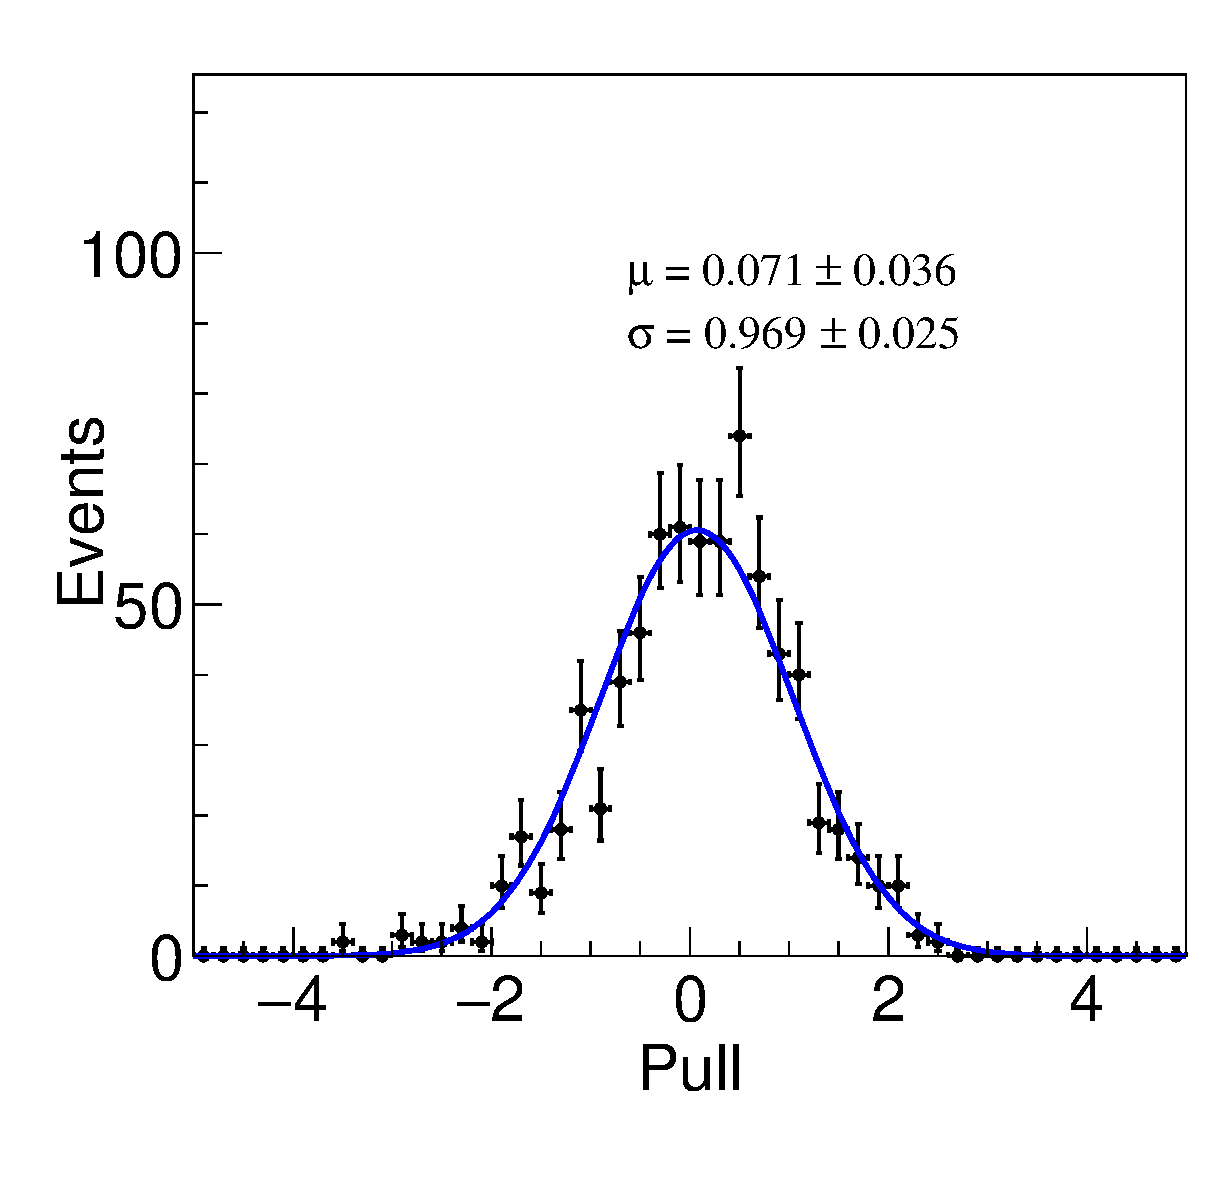
\includegraphics[width = 0.7\linewidth]{dsToPPbar/io/Pull_fit.eps}
    \caption{Pull分布,蓝线为高斯分布。
    }\label{Fig:pull_distribution}
\end{figure}

\subsection{信号灵敏度}
\subsubsection*{$\mathcal{B}(D_{S}^{+} \rightarrow p
\bar{p} e^{+} \nu_{e})$的灵敏度}\label{sec:UL_ds_ppbarenu_MC}
在本节,信号的分支比设为0,也就是伪数据中没有混入任何信号样本。基于同样的
拟合程序来处理这个伪数据,并按96\%的置信度水平设置衰变分支比的上限。
设上限的方法基于贝叶斯
统计\cite{Bayes2001An, Kendall2004Kendall, Zhu2007Upper},方法的精神简述如下:
当观测事例数$N$,分支比的概率分布为\ref{Equ:Bayes}
\begin{equation}
    \label{Equ:Bayes}
    p(B|N) = \frac{\mathcal{L} (N|B) }{\int \mathcal{L} (N|B_{0}) dB_{0}}
\end{equation}
式中$N$经过事例挑选程序后的事例数,$B$为信号的分支比。
注意到$\mathcal{L}(N|B)$的意义就是固定$B$之后通过拟合程序得到似然值,
因此固定分支比,并让其大小从0到1 变化,并通过方程\ref{Equ:Upperlimit}
来得到分支比的上限$Br^{up}$。
\begin{equation}
    \label{Equ:Upperlimit}
    \int^{upper~limit}_{0}p(B|N)dB = 0.9
\end{equation}

拟合的结果见图~\ref{fig:Catefit_mc_up},相应的分支比大小为
$(2.9 \pm 4.2)\times 10^{-5}$,没有显著性的信号,符合我们的预期,从而
按置信度90\%得到分支比的上限为$(1.36 \times 10^{-4})$ 。
\begin{figure}[htbp]
    \centering
    \begin{overpic}[width = 1.0 \linewidth]{dsToPPbar/io/Catefit_mc_up.eps}
        \put(23, 26) {\scalebox{0.9}{\color{juhong} (MC) } }
        \put(57, 26) {\scalebox{0.9}{\color{juhong} (MC) } }
        \put(91, 26) {\scalebox{0.9}{\color{juhong} (MC) } }
    \end{overpic}
    \caption{拟合伪数据中
        $D_{s}^{-}$不变质量谱的结果。其中蓝色的实线表示总的拟合结果,
        黑色的带误差棒的点代表伪数据,红色的点虚线是信号形状。
        }\label{fig:Catefit_mc_up}
\end{figure}


\begin{figure}[htbp] % upper limit Ds->ppbar enu
    \centering
    \begin{overpic}[width = 0.9 \linewidth]{dsToPPbar/io/UP_2DFit.eps}
        \put(68, 58) {\scalebox{1.2}{\color{juhong} (MC)}}
    \end{overpic}
    \caption{变动分支比得到的似然函数曲线。
    }\label{fig:upperlimit_遍举}
\end{figure}


\subsubsection*{研究$\mathcal{B}(D_{S} \rightarrow
X(p\bar{p}) e^{+} \nu_{e}, X \rightarrow p \bar{p})$的上限}
分析的一个重要的动机是研究$p\bar{p}$的共振态。本小节通过研究的
$\mathcal{B}(D_{s}^{+} \to X(p\bar{p}) e^{+} \nu_{e})$
上限来获取数据中探测共振态$X(p\bar{p})$的敏感度。研究基于遍举 蒙特卡洛样本,
通过联合$M(D_{s}^{-})$和$M(p\bar{p})$进行二维拟合得到信号数,进而确定
分支比或者其上限。
在这个二维拟合过程中,信号
蒙特卡洛样本的形状仍然用模拟形状来描述,其中$X(p\bar{p})$的宽度和质量的输入值分别为
1834 MeV$/c^{2}$ and 68 MeV。同时拟合三个标记道的结果如图\ref{fig:UP_D_Xenu}
所示。同样的,我们依旧可以考虑只对$M(D_{s}^{-})$进行拟合,
两者的主要区别为:
\begin{itemize}
    \item 一维拟合。为了得到衰变$D_{s}^{+} \to
        X(p\bar{p}) e^{+} \nu_{e}, X(p\bar{p}) \to p \bar{p}$的分支比上限,
        我们做了如下假设,所有的观测到的来自$D_{s}^{+}$的$p\bar{p}$对都是
        通过中间共振态$X(p\bar{p})$衰变而来。这样假设的合理性在于数据中没有
        明显的信号,故选择变动共振态的分支比扫描似然值获取上限,这就是假设的
        数学基础。故可以得到小结\ref{sec:UL_ds_ppbarenu_MC}同样的结果。
    \item 二维拟合。 这个方法能直接得到的$D_{s}^{+} \to
        X(p\bar{p})e^{+}\nu_{e},~X(p\bar{p})\to p\bar{p}$的分支比。由于
        二维分布能提供更多的数据,故我们期待二维拟合给出更高的灵敏度。
        分支比相应的在90\%置信度下的上限为$1.61 \times 10^{-4}$。总的拟合在
        $M(p\bar{p})$和$M(D_{s}^{-})$维度上的投影
        见图\ref{Fig:2Dfit}。通过变动分支比,得到的似然值曲线
        为\ref{fig:UP_D_Xenu}。
\end{itemize}


\begin{figure}
    \mbox{%
        \begin{overpic}[width = 7 cm]{dsToPPbar/io/mDs_total.eps}
            \put(71, 55) {\scalebox{0.9}{\color{juhong} (MC)}}
        \end{overpic}
        \begin{overpic}[width = 7 cm]{dsToPPbar/io/mPP_total.eps}
            \put(71, 55) {\scalebox{0.9}{\color{juhong} (MC)}}
        \end{overpic}
    }
    \caption{同时对三个标记道进行二维拟合的结果。
    蓝色的实线为总的拟合结果,红色的点虚线是信号形状,绿线分别是三个标记
    道的本底形状。
    }\label{Fig:2Dfit}
\end{figure}
\begin{figure}[htbp]
    \centering
    \mbox{%
        \begin{overpic}[width = 8 cm]{dsToPPbar/io/UP.eps}
            \put(67, 50) {\scalebox{1.2}{\color{juhong} (MC)}}
        \end{overpic}
    }
    \caption{从0开始变动分支比。图中的曲线为扫描得到的似然曲线,红色
    箭头的位置表示似然曲线总积分的90\%部分,也就是90\%置信度下分支比的上限。
        }\label{fig:UP_D_Xenu}
\end{figure}

两种方法结果的比较 
\begin{itemize}
    \item \textbf{上限}
        二维拟合能得到更低的上限,表现要稍优于一维拟合。两种方法得到的分支
        比上限分别是$1.61 \times 10^{-4}$、$1.64 \times 10^{-4}$。
    \item \textbf{系统误差}
        二维拟合的系统误差较大,增加了新的系统误差来源:共振态形状的
        不确定性包括$X(p\bar{p})$的质量和宽度、$B(X(p\bar{p})\to p\bar{p})$
        和本底形状的不确定性。
        与之相比,一维拟合的系统误差较小。
\end{itemize}
综合考虑,我们选择利用一维拟合$M(D_{S}^{-})$分布来决定信号产额或分支比上限。
\subsection{测量结果}\label{sec:result}
\subsubsection{信号产额}
在拟合的过程中,我们通过信号蒙特卡洛样本的形状卷积一个高斯分布以描述信号的形状,
高斯函数的参数,中心值和误差通过拟合单标记的$M(\Dsm)$来得到,
本底的形状则通过\textbf{RooKeyPdf}直接从混合蒙特卡洛样本中得到。
拟合的结果见图\ref{fig:data_Ds}。
\begin{figure}[htbp]
    \centering
        \begin{overpic}[width = 1.0 \linewidth]{dsToPPbar/Fit_Nom.eps}
            \put(21, 23){\scalebox{1.0}{\color{juhong} (data)} }
            \put(55, 23){\scalebox{1.0}{\color{juhong} (data)} }
            \put(90, 23){\scalebox{1.0}{\color{juhong} (data)} }
        \end{overpic}
    \caption{拟合$M(D_{s}^{-})$的结果。蓝色的实线为总的拟合结果,
    红色和绿色的点虚线分别为信号和本底的形状。
    }\label{fig:data_Ds}
\end{figure}
各个标记道中得到的信号数见表\ref{tab:data_yields},相应的分支比为
$( 5.0 ^{+ 6.3}_{-4.4} ) \times 10^{-5}$。
\begin{table}[htbp]
    \caption{各个标记道中拟合得到的信号数}\label{tab:data_yields}
    \begin{center}
        \begin{tabular} {p{0.5\linewidth} p{0.3\linewidth}}
            \toprule
            标记道 & 信号数 \\
            \midrule
            $K_{S}^{0}K^{-}$               & $0.3 ^{+0.4}_{-0.3}$ \\
            $K^{+} K^{-} \pi^{-}$          & $1.4 ^{+1.8}_{-1.3}$ \\
            $K_{S}^{0}K^{+}\pi^{-}\pi^{-}$ & $0.1 \pm 0.1$\\
            \bottomrule
        \end{tabular}
    \end{center}
\end{table}
\subsection{信号分支比的上限}
由于信号的显著性仅为1$\sigma$,本文将在显著性水平$90\%$对信号的分支比求上限。
求上限时,一个棘手的问题是如何处理系统误差。部分系统误差会直接影响拟合数据
时的似然函数,有些则是间接的。比如,本底形状的不确定性则会直接改变似然函数,
另一些因素,比如粒子鉴别的系统误差,则会通过影响信号数的估计间接的改变似然值。
本文利用文献\cite{K.Stenson:2006}的方法处理后者,将影响信号产额的系统误差吸收
到上限的估计之中。下面简要的叙述这一个方法,
通过拟合数据得到的似然值为$L(n)$,称之为原始似然函数,
接着通过卷积的方法吸收信号数的系统误差
如式~\ref{eq:smear}:
\begin{equation}
    \label{eq:smear}
    \mathcal{L}(n)  \varpropto \int _{0} ^{1} L( n \cdot
    \frac{\epsilon}{\epsilon_{0}}) \
    e^{-\frac{{(\epsilon -  \epsilon_{0})}^{2}}
        {2 \sigma_{\epsilon}^{2}}
    } d \epsilon
\end{equation}
式中$\epsilon_{0}$是上文求得的双标记效率,
$\sigma_{\epsilon}$是效率的系统误差。
原始的似然曲线和经过卷积后的似然曲线见图~\ref{fig:prob},
通过积分求90\%的区间后便得到了分支比的上限
\begin{equation}
    \mathcal{B}(D_{s}^{+} \to p \bar{p} e^{+} \nu_{e}) < 1.92 \times
    10^{-4} \notag
\end{equation}

\begin{figure}[htbp]
    \centering
    \begin{overpic}[width = 0.8 \linewidth]{dsToPPbar/prob.eps}
        \put(67, 60){\scalebox{1.0}{\color{juhong} (data) }}
    \end{overpic}
    \caption{似然函数曲线。蓝色和红色和实线分别表示原始似然函数和卷积后
    的似然函数曲线。
    }\label{fig:prob}
\end{figure}



\subsection{系统误差研究}
本文分两种情况研究系统误差
\begin{itemize}
    \item \textbf{I}: 直接影响似然曲线, 比如本底形状;
    \item \textbf{II}: 间接影响似然曲线, 比如寻迹、粒子鉴别。
\end{itemize}
这两类系统误差有明显的不同,
第\textbf{II}类系统误差通过卷积高斯被吸收到上限的估计中,
但是第\textbf{I}类显然不能。

对第类系统误差的讨论见小节\ref{sec:deal_with_background},
比如本底形状系统误差的一个来源是\textbf{RooKeyPdf}类中一个参数``rho''的取值,
这里在1--4之间变动的``rho''的值,每种取值得到的上限列在表\ref{tab:vary_rho}
中。出于保守估计,本文选择其中最大的值作为上限。
\begin{table}[htbp]
    \caption{``rho''的取值对上限的影响。}%
    \label{tab:vary_rho}
    \begin{center}
        \begin{tabular} {c  c c c c c c c }
            \toprule 
            rho  &  1.0 & 1.5 & 2.0 & 2.5 & 3.0 & 3.5 & 4.0 \\
            \midrule  
            UL ($10^{-4}$) & 1.90 & 1.91 & 1.91 & 1.92 & 1.92 & 1.92
            &1.92 \\
            \bottomrule
        \end{tabular}
    \end{center}
\end{table}

\subsection{小结}
采用盲分析方法,本文对伪数据进行了充分研究,决定了实验方案和所有的事例选择
条件,最终选择观测量--$M(D_{s}^{-})$,作为决定信号产额的唯一观测量。
为了验证观测量的合理性,本节比较了两个方法--一维拟合与二维拟合,其中二维拟合
同时考虑了$M(D_{s}^{-})$和$M(p\bar{p})$。
综合考虑到灵敏度和系统误差,本文发现二维拟合对结果的提高极其有限但是又带来
了较大的系统误差,故本文坚持采用一维拟合的方案。
打开数据之后,测得信号的分支比为
$( 5.0 ^{+ 6.3}_{-4.4} ) \times 10^{-5}$,显著性不足3$\sigma$,考虑到
系统误差,在90\%的置信度下,本文给出为
$\mathcal{B}(D_{s}^{+} \to p \bar{p} e^{+} \nu_{e}) < 2.0\times
10^{-4}$。系统误差的具体研究将在下文给出。 

\section{系统误差的研究}%
\label{sec:Systematic_Uncertainties}
系统误差的来源可以分为四类:
\begin{itemize}
    \item 重建:
    质子的寻迹、质子的粒子鉴别;
    \item 事例选择条件:
        对$MM^{2}$, 质子动量,和电子动量的要求;
    \item 拟合:
        信号形状、本底形状、单标记$D_{s}^{-}$介子产额;
    \item 模型:
        产生子模型。
\end{itemize}

\subsection{重建}
单标记侧的寻迹和粒子鉴别的系统误差和双标记侧的相互抵消,因此重建的系统误差
只有信号侧的质子寻迹和鉴别的系统误差。质子的粒子鉴别的系统误差在
小节~\ref{Sec:Correction_of_Efficiency}已经进行了研究,系统误差的大小为
2.2\%。
对于质子寻迹的系统误差,本文利用数据和伪数据中的质子寻迹效率,对信号蒙特卡洛样本进行加权
平均,所用到的公式是~\ref{eq:track-error},
\begin{equation}
    \begin{aligned}
        \label{eq:track-error}
        &\epsilon(reweight) = \sum_{i}  \frac{n_{i} \epsilon_{i}(data) / 
        \epsilon_{i} (MC) }{N} \notag  \\
        & \delta_{i}  =  \frac{\epsilon_{i}(data) -
        \epsilon(MC)}{\epsilon_{i}(data)}  \notag  \\
        &\bar{\delta}  =  \frac{\epsilon(reweight) -
        \epsilon(MC)}
        {\epsilon (reweight)}
    \end{aligned}
\end{equation}
式中$\epsilon_{i}(data)$和
$\epsilon_{i}(MC)$分别是数据和伪数据 
中质子的寻迹效率,本文采用文献~\cite{HaoXq:ProtonPID}中的结果,
相应的大小列在表~\ref{tab:proton-efficiency}之中,
$\epsilon(reweight)$则是经过加权后的信号效率。
信号蒙特卡洛样本按正反质子的动量大小分成$5\times5$个区间,
如表~\ref{tab:ratios}所示。\ref{tab:evts}. 
在下面的分析中,将按这25个区间进行加权得到总效率,进而决定质子寻迹的系统
误差。首先考虑到第$i$个区间内的效率等于
\begin{equation}
    \epsilon_{i}(p\bar{p}) = \epsilon_{n}(p) \epsilon_{m}(\bar{p})
    \notag
\end{equation}
式中质子在$n$个动量区间,反质子则在$m$个动量区间,这一个区间内的
同时寻找到正反质子对的效率为$\epsilon_{i}(P\bar{P})$。
在之后的公式里,脚标$p\bar{p}$将被省略。
\begin{table}[htbp] %efficiency
    \caption{数据和蒙特卡洛样本中的质子寻迹效率差异。
    }%
    \label{tab:proton-efficiency}
    \begin{center}
        \begin{tabular} {c c c c c c}
            \toprule
            $p_{t}(p) (MeV)$  &  100--200 & 200--300 & 300--400 
            & 400--500 & 500--600 \\
            \midrule
            $1-  \frac{\epsilon_{MC}}{\epsilon_{data}}  (\%) $  &
            $ -2.3 \pm  2.4  $ & $ -0.27 \pm 1.1  $  &
            $ -0.34 \pm 0.42 $ & $ - 0.28 \pm 0.32 $ & 
            $ -0.09 \pm 3.7 $  \\
            \midrule
            $p_{t}(\bar{P}) (MeV)$  &  100--200 & 200--300 
            & 300--400 & 400--500 & 500--600 \\
            \midrule
            $1-  \frac{\epsilon_{MC}}{\epsilon_{data}} (\%)$  &
            $ -7.6 \pm  5.3  $ & $ -0.96 \pm 1.3  $  &
            $ -0.36 \pm 1.1 $ & $ - 1.2 \pm 1.2 $ & 
            $ -0.6 \pm 2.6 $ \\
            \bottomrule
        \end{tabular}
    \end{center}
\end{table}
\begin{table}[htbp] %ratio
    \caption{每个区间内事例数比例。按质子(反质子)的动量划分区间。
    信号蒙特卡洛样本总大小为35000个事例。}%
    \label{tab:ratios}
    \centering
    \begin{tabular} {c  c |  c c  c c c}
        \toprule
        \multicolumn{2}{c}{\multirow{2}{*}{$\frac{n_{i}}{N}$~(\%)}}
        & \multicolumn{5}{|c}{$p_{t}(\bar{P}) (MeV)$} \\ 
        & &  100--200 & 200--300 & 300--400 & 400--500 & 500--600 \\
        \midrule
        \multirow{5}{*}
        {\rotatebox{90}{$p_{t}(\bar{P}) (MeV)$ }} 
        &  100--200 & 1.34  & 7.79  & 3.64 & 0.48 & 0.011 \\
        & 200--300      & 8.84  & 38.9  & 13.4 & 1.48 & 0.008 \\
        & 300--400      & 4.49  & 13.7  & 3.38 & 0.149 & 0.00 \\
        &400--500     & 0.625 & 1.62  & 1.18 & 0.00 & 0.00 \\
        &500--600      & 0.008 & 0.011 & 0.00 & 0.00 & 0.00 \\
        \bottomrule
    \end{tabular}
    \begin{tabular} {c  c |  c c  c c c}
        \toprule
        \multicolumn{2}{c}{\multirow{2}{*}{$n_{i}$}}
        & \multicolumn{5}{|c}{$p_{t}(\bar{P}) (MeV)$} \\ 
        & &  100--200 & 200--300 & 300--400 & 400--500 & 500--600 \\
        \midrule
        \multirow{5}{*}
        {\rotatebox{90}{$p_{t}(\bar{P}) (MeV)$}} 
        & 100--200 & 475  & 2764  & 1292 & 172 & 4 \\
        & 200--300 & 3138 & 13814 & 4743 & 526  & 3 \\
        & 300--400 & 1594 & 4873  & 1198 & 53 & 0 \\
        & 400--500 & 222  & 574   & 42   & 0  & 0 \\
        & 500--600 & 3    & 4     & 0 & 0  & 0 \\
        \bottomrule
    \end{tabular}
\end{table}

综上所述,可以得到 
\begin{equation}
    \bar{\delta} = 1.2 \% \notag
\end{equation}
$\bar{\delta}$的误差由方程\ref{eq:track-corr-error}得到
\begin{equation}
    \begin{aligned}
        \label{eq:track-corr-error}
        \Delta \bar{\delta }^{2} & = 
        \sum_{i,j} 
        \frac{\partial \bar{\delta }} {\partial \delta_{i}} \cdot 
        \frac{\partial \bar{\delta }} {\partial \delta_{j}} \cdot 
        \delta_{i} \delta_{j}  
        \notag \\
        &= \sum_{i,j}  \frac{n_{i}}{N} \frac{n_{j}}{N}
        cov_{i,j}   \Delta  \delta_{i} \Delta  \delta_{j} 
    \end{aligned}
\end{equation}
式中$cov_{i,j}$是$\delta_{i}$和$\delta_{j}$的相关系数。
如果假设$cov_{i,j}=0$,也就是各个区间内的样本相互独立将得到
$ \Delta \bar{\delta } = 1.0\%$;如果做最保守的估计,假设各个区间
之间完全相关,也就是$cov_{i,j}=1$,那么将得到较大的误差,大小为 
\begin{equation}
    \Delta \bar{\delta} = 2.9\% \notag
\end{equation}
因此出于保守估计,这项系统误差定为2.9\%.

\subsubsection{电子寻迹}
在这些分析中,电子寻迹的系统误差为0。按前文所述,只有找到一对正反
质子对之后才考虑寻找电子的径迹。不管是否能够找到电子的径迹,这个事例
都将被保留,因此电子寻迹不会贡献任何系统误差。

\subsection{事例选择条件}
由于仅有约5\%是事例中能够找到电子径迹,在这部分事例中,本文要求电子的动量
小于90MeV,带来的系统误差约为1\%,对总的事例的系统误差的贡献可以忽略不记。
除了对电子动量的选择条件,本文还要求
丢失不变质量大于0${(GeV/c^{2})}^{2}$,这项系统误差的来源在于数据和蒙特卡洛样本之间
的$MM^{2}$的分辨率不同。分辨率由带电径迹的
探测器分辨决定。为了补偿这种差异,本文选择在蒙特卡洛信号形状的基础上卷积一个高斯
函数来描述数据中的$MM^{2}$形状,高斯函数参数的不确定性带来的相对变化
作为系统误差,在章节\ref{sec:cut-on-MM}中做了详细研究,系统误差定为1.0\%。

\subsection{拟合方法}
和单标记道有关的系统误差包括:信号形状、本底形状和拟合范围。
为了估计信号形状带来的系统误差,本文变动拟合模型中的信号形状,
从模拟形状变为双高斯函数,信号产额仅仅变化0.5\%,因此本文选择把0.5\%作为
信号形状带来的系统误差。同样的,本文变化本底形状,用更高阶的切比雪夫多
项式替代模型中的本底形状,并信号产额的变化作为系统误差。
为了保守估计拟合范围带来的系统误差,本文5MeV的范围内浮动拟合范围的上下限,
信号产额的最大变化作为系统误差。
这三项系统误差的大小总结在表\ref{tab:sys-uncerainty-fitting}中。

\begin{table}[htbp]
    \caption{来自拟合的系统误差}%
    \label{tab:sys-uncerainty-fitting}
    \centering
    \begin{tabular}{p{0.2 \linewidth} p{0.2 \linewidth} p{0.2 \linewidth} 
        p{0.2 \linewidth}}
        \toprule
        误差来源 & 拟合范围 & 本底形状 & 信号形状\\
        \midrule
        误差大小 & 0.3\%  & 0.2\%  & 0.5 \%  \\ 
        \bottomrule
    \end{tabular}
\end{table}
这三项系统误差总和为0.7\%。
\subsection{产生子模型}
在正则模型里,本文假定$D_{s}^{+}$介子直接衰变到
$p\bar{p}e^{+} \nu_{e}$, 产生的$p\bar{p}$对形成S波。
另外,还有很多其他的合理的模型,比如
$p\bar{p}$可能来自中间共振态$X(p\bar{p})$,假定我赝标量粒子,宽度和质量
分别为
1834 MeV$/c^{2}$、68 MeV。两个模型中的信号效率的相对差异为$18\%$。
此外中间共振态的宽度和质量也会影响效率,在小节\ref{uncertainties for Xpp}
中详细地研究了这项系统误差,
约为2.5\%

\subsection{本底}%
\label{sec:deal_with_background}
在获取上限的过程中,本底带来的系统误差不能简单的通过公式~\ref{eq:smear}
吸收到上限的估计之中。如果变动本底的形状,将会得到一系列上限的估计值。
下文将详细叙述本底形状的变化方式。在小结\ref{sec:dt-efficiency}中,
本底形状借助于工具\textbf{RooKeyPdf}得到,最大的确定性来自参数``rho''
的设置值,本文把``rho''在1--4之间浮动,将得到一系列形状,接着根据每种
形状估计分支比上限,并把最大的上限估计值作为最终的实验结果。

\subsection*{系统误差研究的总结}
至此,本文已经研究了所有的系统误差,每项系统误差的具体数值列在
表\ref{tab:short_summary}中。

\begin{table}[htbp]
    \caption{系统误差的总结}%
    \label{tab:short_summary}
    \centering
    \begin{tabular}{p{0.45 \linewidth} p{0.45 \linewidth} }
        \toprule
        来源 & 误差 ($\%$) \\ 
        \midrule
        单标记产额       & 1.0 \\
        寻迹$^{a}$       & 2.9 \\
        粒子鉴别         & 2.2 \\
        对$MM^{2}$的要求 & 1.0 \\
        产生子模型$^{b}$ & 18 \\
        \midrule
        总和 & 19 \\
        \bottomrule
    \end{tabular}
\end{table}

